\documentclass[a4paper]{book}
\usepackage[
    a4paper,heightrounded,includefoot,includemp,
    top=4cm,bottom=4cm,outer=1cm,inner=3.5cm,
    marginparwidth=4cm,
]{geometry}
\usepackage{graphicx}
\usepackage{hyperref}
\usepackage{lettrine}
\usepackage{polyglossia}
\usepackage{tabularx}
\usepackage{titlesec}
\usepackage{titling}
\usepackage{wrapfig}
%\usepackage{showframe}

\setmainlanguage{english}
\setotherlanguage{greek}
\setotherlanguage{latin}
\newfontfamily{\greekfont}{DejaVuSerif}
\newfontfamily{\romanfont}{Nimbus Roman}
\newfontfamily{\liturgicalfont}{Junicode}
\selectlanguage{latin}

\pagestyle{plain}
\setcounter{tocdepth}{1}
%\setcounter{secnumdepth}{0}
\renewcommand{\numberline}[1]{}

\titleclass{\chapter}{straight}
\titleformat{\chapter}[hang]
    {}{}{0pt}{\filcenter\romanfont\huge\MakeUppercase}
\titleformat{\section}[hang]
    {}{}{0pt}{\filcenter\romanfont\large\MakeUppercase}
\titleformat{\subsection}[hang]
    {}{}{0pt}{\filcenter\romanfont\itshape\MakeUppercase}
\titlespacing{\section}{0pt}{1em}{0.5em}
\titlespacing{\subsection}{0pt}{1em}{0.5em}
\addto{\captionsenglish}{\renewcommand\contentsname{Index}}

\newcommand{\persona}[1]{
    \makebox[1em][c]{\liturgicalfont{}#1.}
}
\newcommand{\bibliafmt}[1]{{\bfseries\itshape{}#1}}
\newcommand{\biblia}[1]{\bibliafmt{#1}}
\newcommand{\versiculum}{\persona{℣}}
\newcommand{\responsorium}{\persona{℟}}
\newcommand{\sacerdos}{\persona{S}}
\newcommand{\minister}{\persona{M}}
\newcommand{\cross}{{\liturgicalfont\huge\raisebox{-0.2em}{᛭}}}
\newcommand{\sinus}{\directio{sinus}}
\newcommand{\alternatim}[1]{{\setlength{\parskip}{0pt}#1}}
\newcommand{\initialis}[2][2]{\lettrine[lines=#1]{\romanfont\bfseries{}#2}{} }
\newcommand{\directio}[1]{[\hspace{0.1em}\textit{#1}\hspace{0.2em}]}
\newcommand{\proprius}[1]{\directio{proprius: #1}}

\newcommand{\divisio}{{
    \setlength{\parskip}{0pt}
    \vspace{0.25em}
    \hspace{\fill}\rule{0.33\textwidth}{.2pt}\hspace*{\fill}
    \vspace{0.25em}
}}

\title{Missale}
\date{1962}

\begin{document}
    \frontmatter
    \titlespacing{\chapter}{0pt}{\baselineskip}{\baselineskip}
    \newgeometry{margin=0pt}
\begin{titlepage}
    \centering
    \flushbottom
    \vspace*{-2em}
    \vspace*{\stretch{1}}

    \vspace*{\stretch{3}}

    {\romanfont\fontsize{60}{60}\selectfont\MakeUppercase{\thetitle}}

    \vspace{\stretch{3}}

    \vspace{\stretch{2}}

    
\includegraphics[width=0.4\textwidth]{img/chi_rho.png}
    \vspace{-0.5em}

    \vspace{\stretch{2}}

    \vspace{\stretch{4}}

    {\romanfont\fontsize{32}{32}\selectfont\uppercase{Ritus Romanus}}
    \\[2\baselineskip]

    {\Large\MakeUppercase{\romannumeral\thedate}}
    \\[\baselineskip]

    \vspace{\stretch{1}}
\end{titlepage}
\restoregeometry

    \phantomsection\addcontentsline{toc}{chapter}{\contentsname}
\tableofcontents

\vspace{\fill}

{\let\cleardoublepage\clearpage\chapter*{Glossarium}}

\begin{center}
    \begin{tabularx}{0.75\textwidth}{c@{}XX}
        \versiculum{}   & versiculum   & \cross{} signum crucis \\
        \responsorium{} & responsorium & \bibliafmt{Biblia 1, 2-3} \\
        \sacerdos{}     & sacerdos     & \textit{explanatio} \\
        \minister{}     & minister     & \directio{directio} \\
    \end{tabularx}
\end{center}


\vspace{\fill}

\begin{center}
    \url{https://media.musicasacra.com/pdf/missale62.pdf} \\
    \url{https://archive.org/details/TheLiberUsualis1961}
\end{center}

    \mainmatter
    \titleclass{\chapter}{top}
    \titlespacing{\chapter}{0pt}{0pt}{1em}
    \setlength{\parskip}{0.5em}
    {\let\cleardoublepage\clearpage\chapter{Asperges}}

\section{Benedictio aquae}

\textit{%
    Die dominico, in sacristia praeparato sale et aqua benedicenda, sacerdos
    celebraturus Missam vel alius ad id deputatus, alba vel superpelliceo
    indutus cum stola circa collum, primo dicit:
}

\biblia{Ps. 123, 8}

\versiculum{Adiutorium nostrum in nomine Domini.}
{\setlength{\parskip}{0pt}
\par\responsorium{Qui fecit caelum et terram.}}

\textit{Deinde absolute incipit exorcismum salis.}

\initialis{E}xorcizo te, creatura salis, \ldots

\section{Aspersio aquae benedictae}

\vspace{-0.5\baselineskip}\directio{stans}

\begin{wrapfigure}{r}{0.55\textwidth}
    \centering
    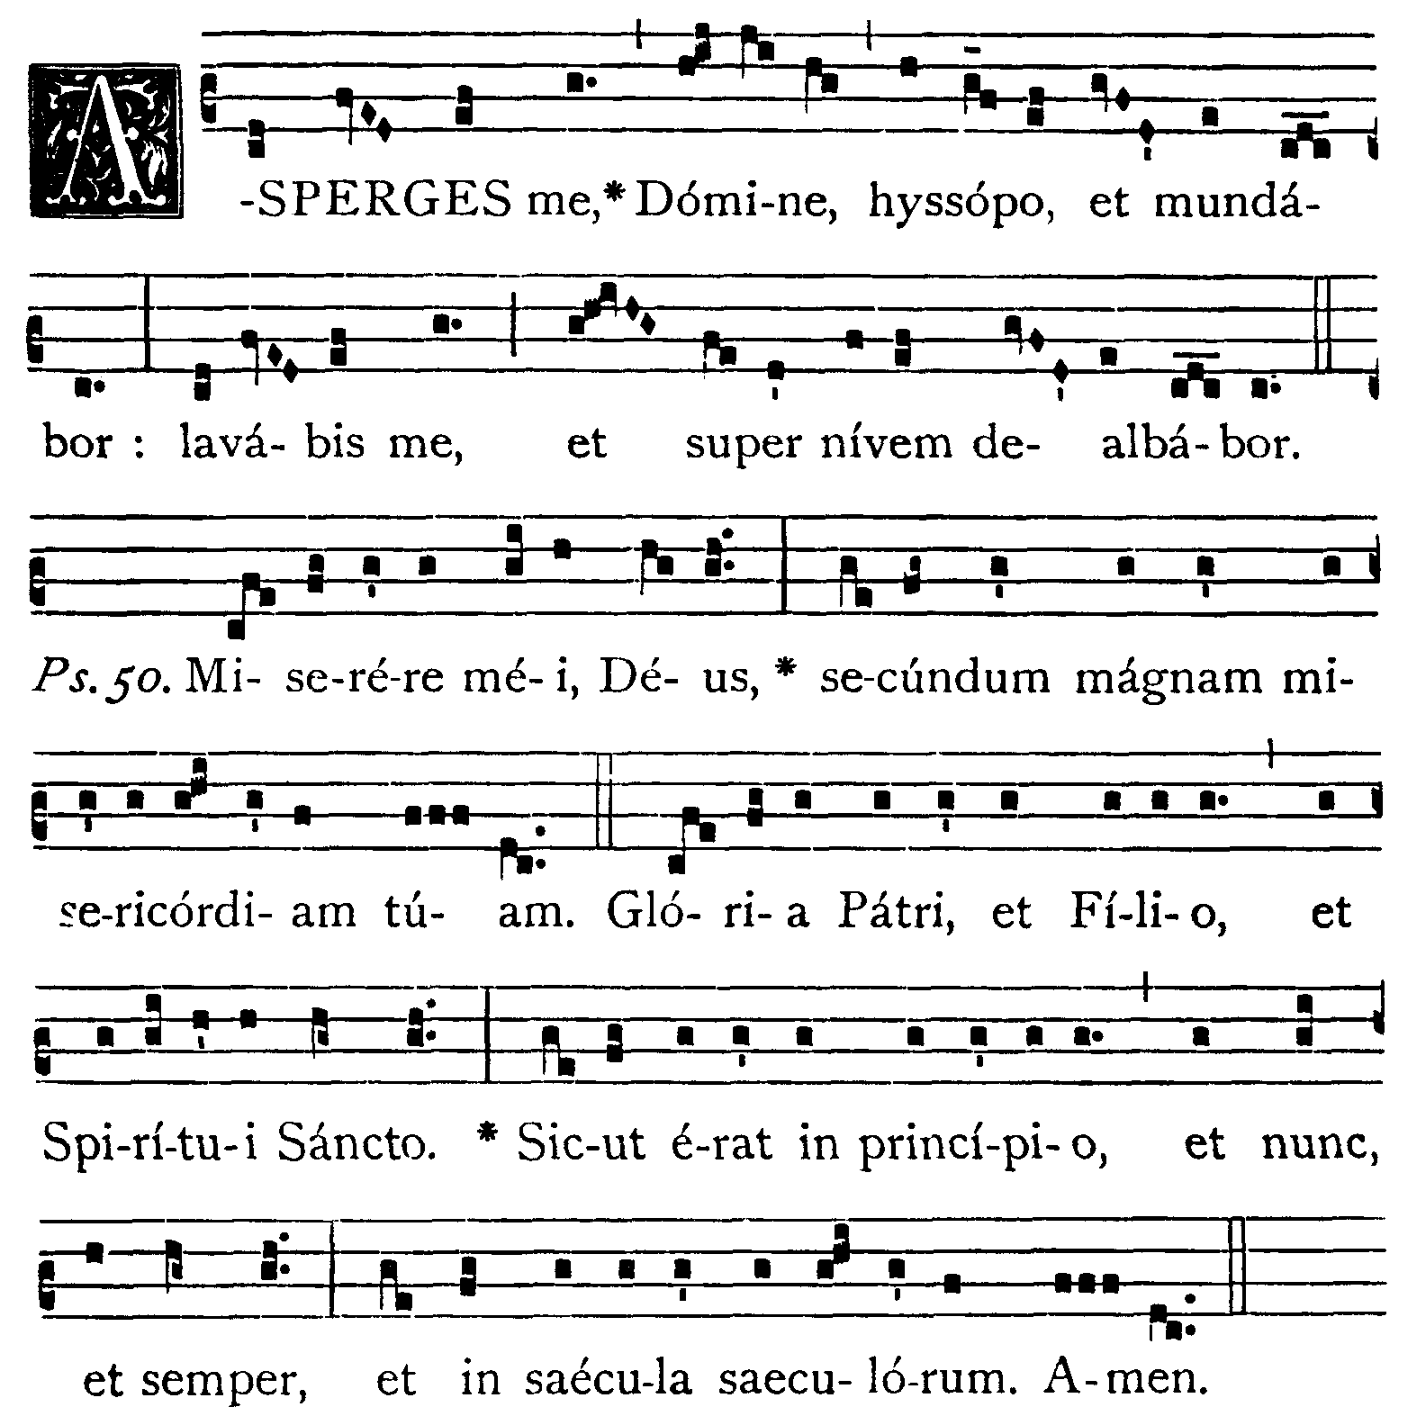
\includegraphics
        [scale=0.3, clip, viewport=1cm 42cm 30cm 49.5cm]
        {img/asperges.png}
\end{wrapfigure}

\textit{Extra tempus paschale sacerdos celebraturus, indutus pluviali coloris
officio convenientis, accedit ad altare, et ibi ad gradus cum ministris
genuflexus, etiam tempore paschali, accipit a diacono aspersorium, et primo ter
aspergit altare, deinde se, et erectus ministros, incipiens antiphonam} Asperges
me.  \textit{Et chorus prosequitur}: Domine, hyssopo, \textit{etc., ut infra.
Interim celebrans aspergit clerum, deinde populum.}

\vspace{\baselineskip}

\begin{tabularx}{\dimexpr\textwidth-\parindent}{@{}p{5em}X@{}}
    \bibliafmt{Ps. 50, 9} &
    Asperges me (Domine) hyssopo et mundabor /
    lavabis me et super nivem dealbabor.
    \\ \noalign{\vspace{1em}}
    \bibliafmt{Ps. 50, 3} &
    Miserere mei, Deus, secundum magnam misericordiam tuam.
    \\ \noalign{\vspace{1em}}
    \bibliafmt{Doxologia \newline minor} &
    \directio{flectens} Gloria Patri, et Filio, et Spiritui Sancto: sicut erat
    in principio, et nunc, et semper, et in saecula saeculorum.  Amen.
    \\
\end{tabularx}

\vspace{\baselineskip}

\divisio

\textit{%
    Tempore Passionis non dicitur Gloria Patris post psalmum Miserere, sed
    repetitur immediate antiphona Asperges Me.
}

\divisio

\directio{stans}

\textit{%
    Finita antiphona supradicto modo, sacerdos, qui aspersit aquam, reversus ad
    altare, stans ante gradus altaris, iunctis manibus, dicat:
}

\versiculum{Ostende nobis, Domine, misericordiam tuam.}
{\setlength{\parskip}{0pt}
\par\responsorium{Et salutare tuum da nobis.}
\par\versiculum{Domine, exaudi orationem meam.}
\par\responsorium{Et clamor meus ad te veniat.}
\par\versiculum{Dominus vobiscum.}
\par\responsorium{Et cum spiritu tuo,}}

Oremus.

\initialis{E}xaudi nos, Domine, sancte Pater, omnipotens aeterne Deus: et
mittere digneris sanctum Angelum tuum de caelis; qui custodiat, foveat,
protegat, visitet atque defendat omnes habitantes in hoc habitaculo.  Per
Christum Dominum nostrum.

\responsorium{Amen.}

\vfill
\begin{figure}[h]
    \centering
    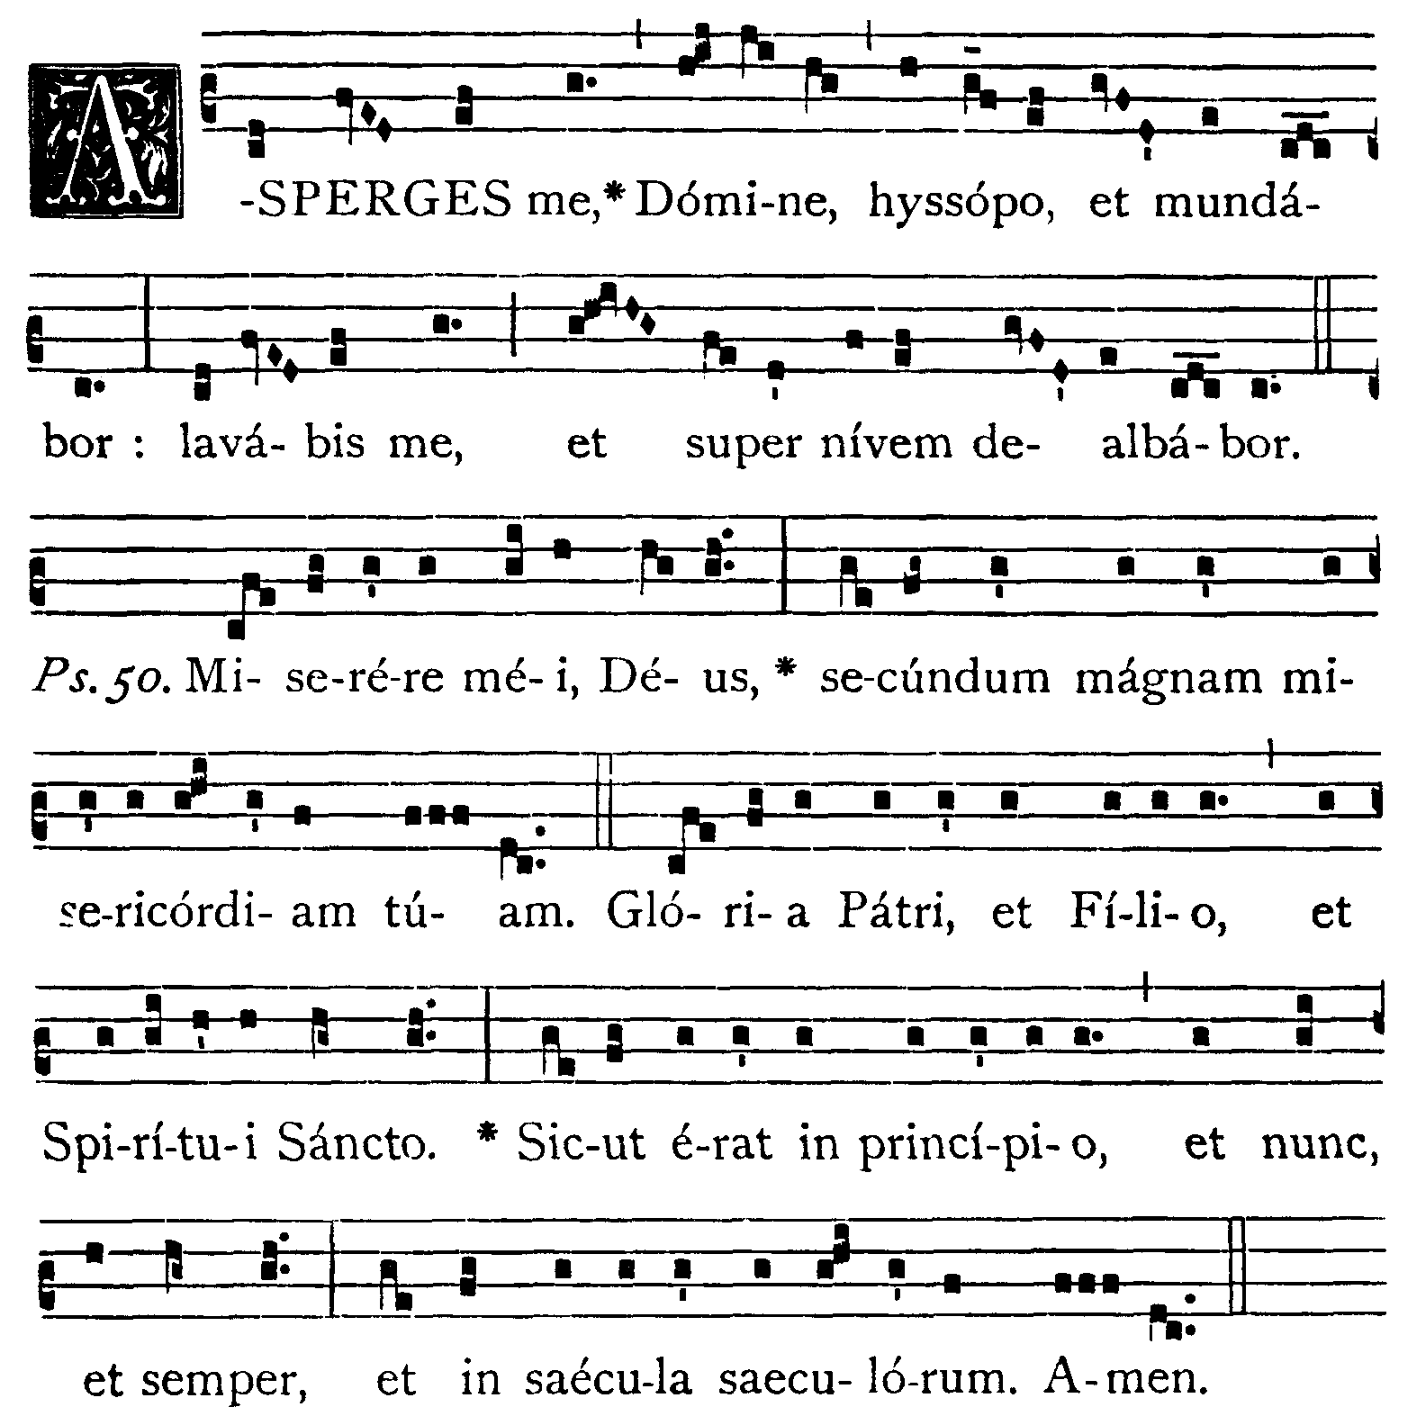
\includegraphics[scale=0.3]{img/asperges.png}
\end{figure}
\vfill

    {\let\cleardoublepage\clearpage\chapter{Missa Catechumenorum}}

\directio{genuflectens}

\textit{%
    Sacerdos paratus cum ingreditur ad altare, facta illi debita reverentia,
    signat se signo crucis a fronte ad pectus, et, nisi peculiari rubrica aliter
    statuatur, clara voce dicit:
}

\initialis[3]{I}n nomine Patri, \cross{} et Filii, et Spiritus Sancti.  Amen.

\hspace{0.5em}\textit{Deinde, iunctis manibus ante pectus, incipit antiphonam:}

\versiculum{Introibo ad altare Dei.}

\textit{Ministri respondent:}

\responsorium{Ad Deum qui laetificat iuventutem meam.}

\textit{Postea alternatim cum ministris dicit sequentem:}

\biblia{Ps. 42, 1-5}

\initialis{I}udica me, Deus, et discerne causam meam de gente non sancta: ab
homine iniquo, et doloso erue me.

\minister{%
    Quia tu es, Deus, fortitudo mea: quare me repulisti, et quare tristis
    incedo, dum affligit me inimicus?
}
\alternatim{
    \par\sacerdos{%
        Emitte lucem tuam, et veritatem tuam: ipsa me deduxerunt, et adduxerunt
        in montem sanctum tuum, et in tabernacula tua.
    }
    \par\minister{%
        Et introibo ad altare Dei: ad Deum qui laetificat iuventutem meam.
    }
    \par\sacerdos{%
        Confitebor tibi in cithara, Deus, Deus meus: quare tristis es, anima
        mea, et quare conturbas me?
    }
    \par\minister{%
        Spera in Deo, quoniam adhuc confitebor illi: salutare vultus mei, et
        Deus meus.
    }
    \par\sacerdos{Gloria Patri, et Filio, et Spiritui Sancto.}
    \par\minister{%
        Sicut erat in principio, et nunc, et semper: et in saecula saeculorum.
        Amen.
    }
}

\textit{Sacerdos repetit antiphonam:}

\versiculum{Introibo ad altare Dei.}
\alternatim{\par\responsorium{Ad Deum qui laetificat iuventutem mean.}}

\textit{Signat se, dicens:}

\versiculum{Adiutorium nostrum \cross{} in nomine Domini.}
\alternatim{\par\responsorium{Qui fecit caelum et terram.}}

\textit{Deinde, iunctis manibus, profunde inclinatus facit confessionem.}

\pagebreak

\divisio

\textit{In Missis defunctorum, et in Missis de Tempore a dominica I Passionis
usque ad feriam V in Cena Domini inclusive, omittitur psalmus} Iudica me, Deus,
\textit{cum} Gloria Patri, \textit{et repetitione antiphonae, sed dicto} In
nomine Patris, Introibo, \textit{et} Adiutorium, \textit{fit confessio, ut
sequitur}:

\divisio

\section{Confiteor}

\initialis{C}onfiteor Deo omnipotenti, beatae Mariae semper Virgini, beato
Michaeli Archangelo, beato Ioanni Baptistae, sanctis Apostolis Petro et Paulo,
omnibus Sanctis, et vobis, fratres: quia peccavi nimis cogitatione, verbo et
opere: (\textit{percutit sibi pectus ter, dicens:}) mea culpa, mea culpa, mea
maxima culpa.  Ideo precor beatam Mariam semper Virginem, beatum Michaelem
Archangelum, beatum Ioannem Baptistam, sanctos Apostolos Petrum et Paulum, omnes
Sanctos, et vos, fratres, orare pro me ad Dominum Deum nostrum.

\textit{Ministri respondent:}

\initialis{M}isereatur tui omnipotens Deus, et, dimissis peccatis tuis, perducat
te ad vitam aeternam.

\textit{Sacerdos dicit:}

\versiculum{Amen.}

\textit{et erigit se.  Deinde ministri repetunt confessionem: et ubi a sacerdote
dicebatur} vobis, fratres, \textit{et} vos, fratres, \textit{a ministris
dicitur} tibi, pater, \textit{et} te, pater.  \textit{Postea sacerdos, iunctis
manibus, facit absolutionem, dicens:}

\initialis{M}iseratur vestri omnipotens Deus, et, dimissis peccatis vestris,
perducat vos ad vitam aeternam.

\responsorium{Amen.}

\textit{Signat se signo crucis, dicens:}

\initialis{I}ndulgentiam, \cross{} absolutionem et remissionem peccatorum
nostrorum tribuat nobis omnipotens et misericors Dominus.

\responsorium{Amen.}
\alternatim{
    \par\textit{Et inclinatus prosequitur:}
    \par\versiculum{Deus, tu conversus vivificabis nos.}
    \par\responsorium{Et plebs tua laetabitur in te.}
    \par\versiculum{Ostende nobis, Domine, misericordiam tuam.}
    \par\responsorium{Et salutare tuum da nobis.}
    \par\versiculum{Domine, exaudi orationem meam.}
    \par\responsorium{Et clamor meus ad te veniat.}
    \par\versiculum{Dominus vobiscum.}
    \par\responsorium{Et cum spiritu tuo.}
}

\textit{Et, extendens ac iungens manus, clara voce dicit:}

\versiculum{Oremus.}

\directio{stans}

\textit{et, ascendens ad altare, dicit secreto:}

\initialis{A}ufer a nobis, quaesumus, Domine, iniquitates nostras: ut ad Sancta
sanctorum puris mereamur mentibus introire.  Per Christum Dominum nostrum.
Amen.

\textit{Deinde, manibus iunctis super altare, inclinatus dicit:}

\initialis{O}ramus te, Domine, per merita Sanctorum tuorum, (\textit{osculatur
altare in medio}) quorum reliquiae hic sunt, et omnium Sanctorum: ut indulgere
digneris omnia peccata mea.  Amen.

\textit{%
    In Missa solemni, quae non sit defunctorum, celebrans, antequam incipiat
    antiphonam ad Introitum, benedicit incensum, dicens:
}

\sacerdos{Ab illo bene\cross{}dicaris, in cuius honore cremaberis.  Amen.}

\textit{%
    Et, accepto thuribulo a diacono, incensat altare, nihil dicens.  Postea
    diaconus, recepto thuribulo a celebrante, incensat illum tantum.
}

\section{Introitus}

\proprius{Introitus}

\textit{%
    Deinde celebrans, signans se signo crucis, incipit antiphonam ad Introitum
    qua finita, iunctis manibus, alternatim cum ministris dicit:
}

\section{Kyrie Eleison}

\begin{wrapfigure}{r}{0.6\textwidth}
    \centering
    \vspace{-0.5\baselineskip}
    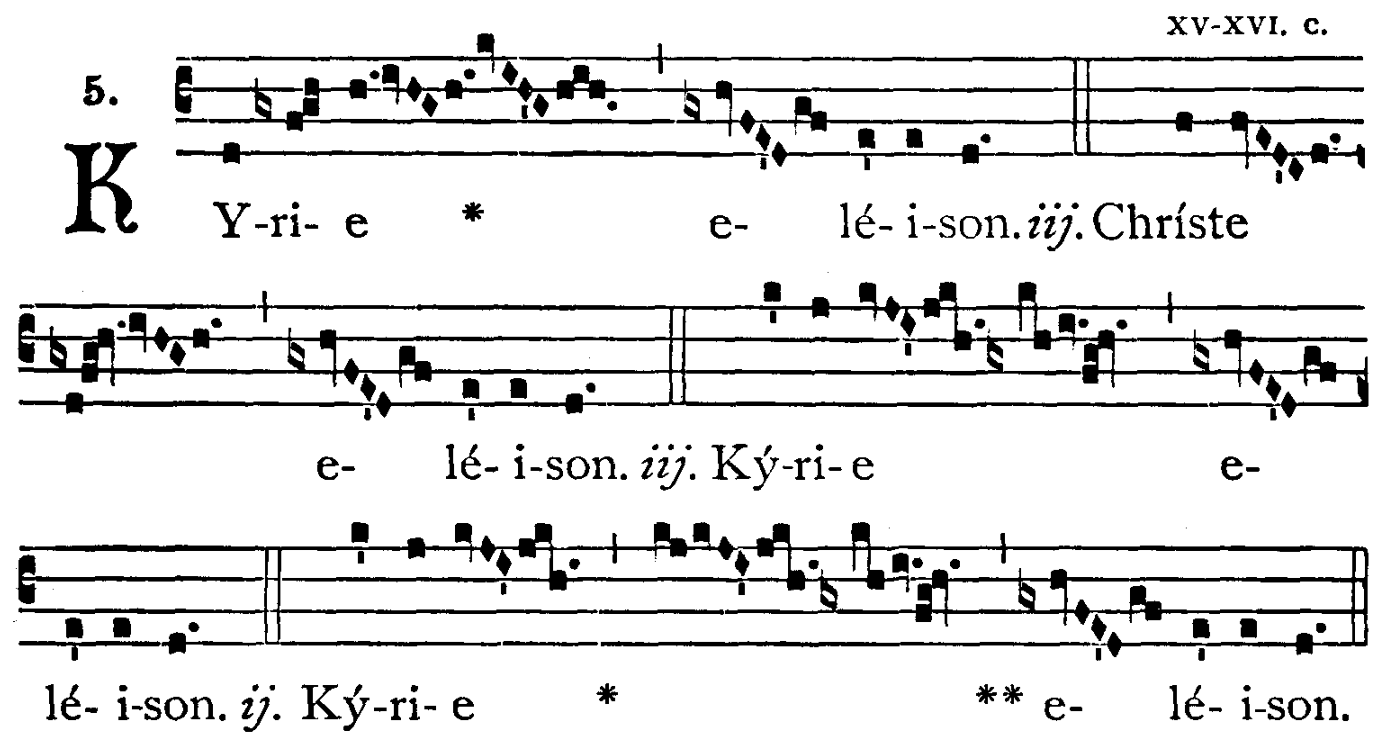
\includegraphics
        [scale=0.3, clip, viewport=2cm 17.5cm 22.5cm 25cm]
        {img/kyrie.png}
\end{wrapfigure}

\initialis{K}yrie, eleison. Kyrie, eleison. \\ Kyrie, eleison. \\
Christe, eleison.  Christe eleison. \\ Christe eleison. \\
Kyrie eleison.  Kyrie eleison. \\ Kyrie eleison.

\section{Gloria in Excelsis}

\begin{wrapfigure}{r}{0.5\textwidth}
    \centering
    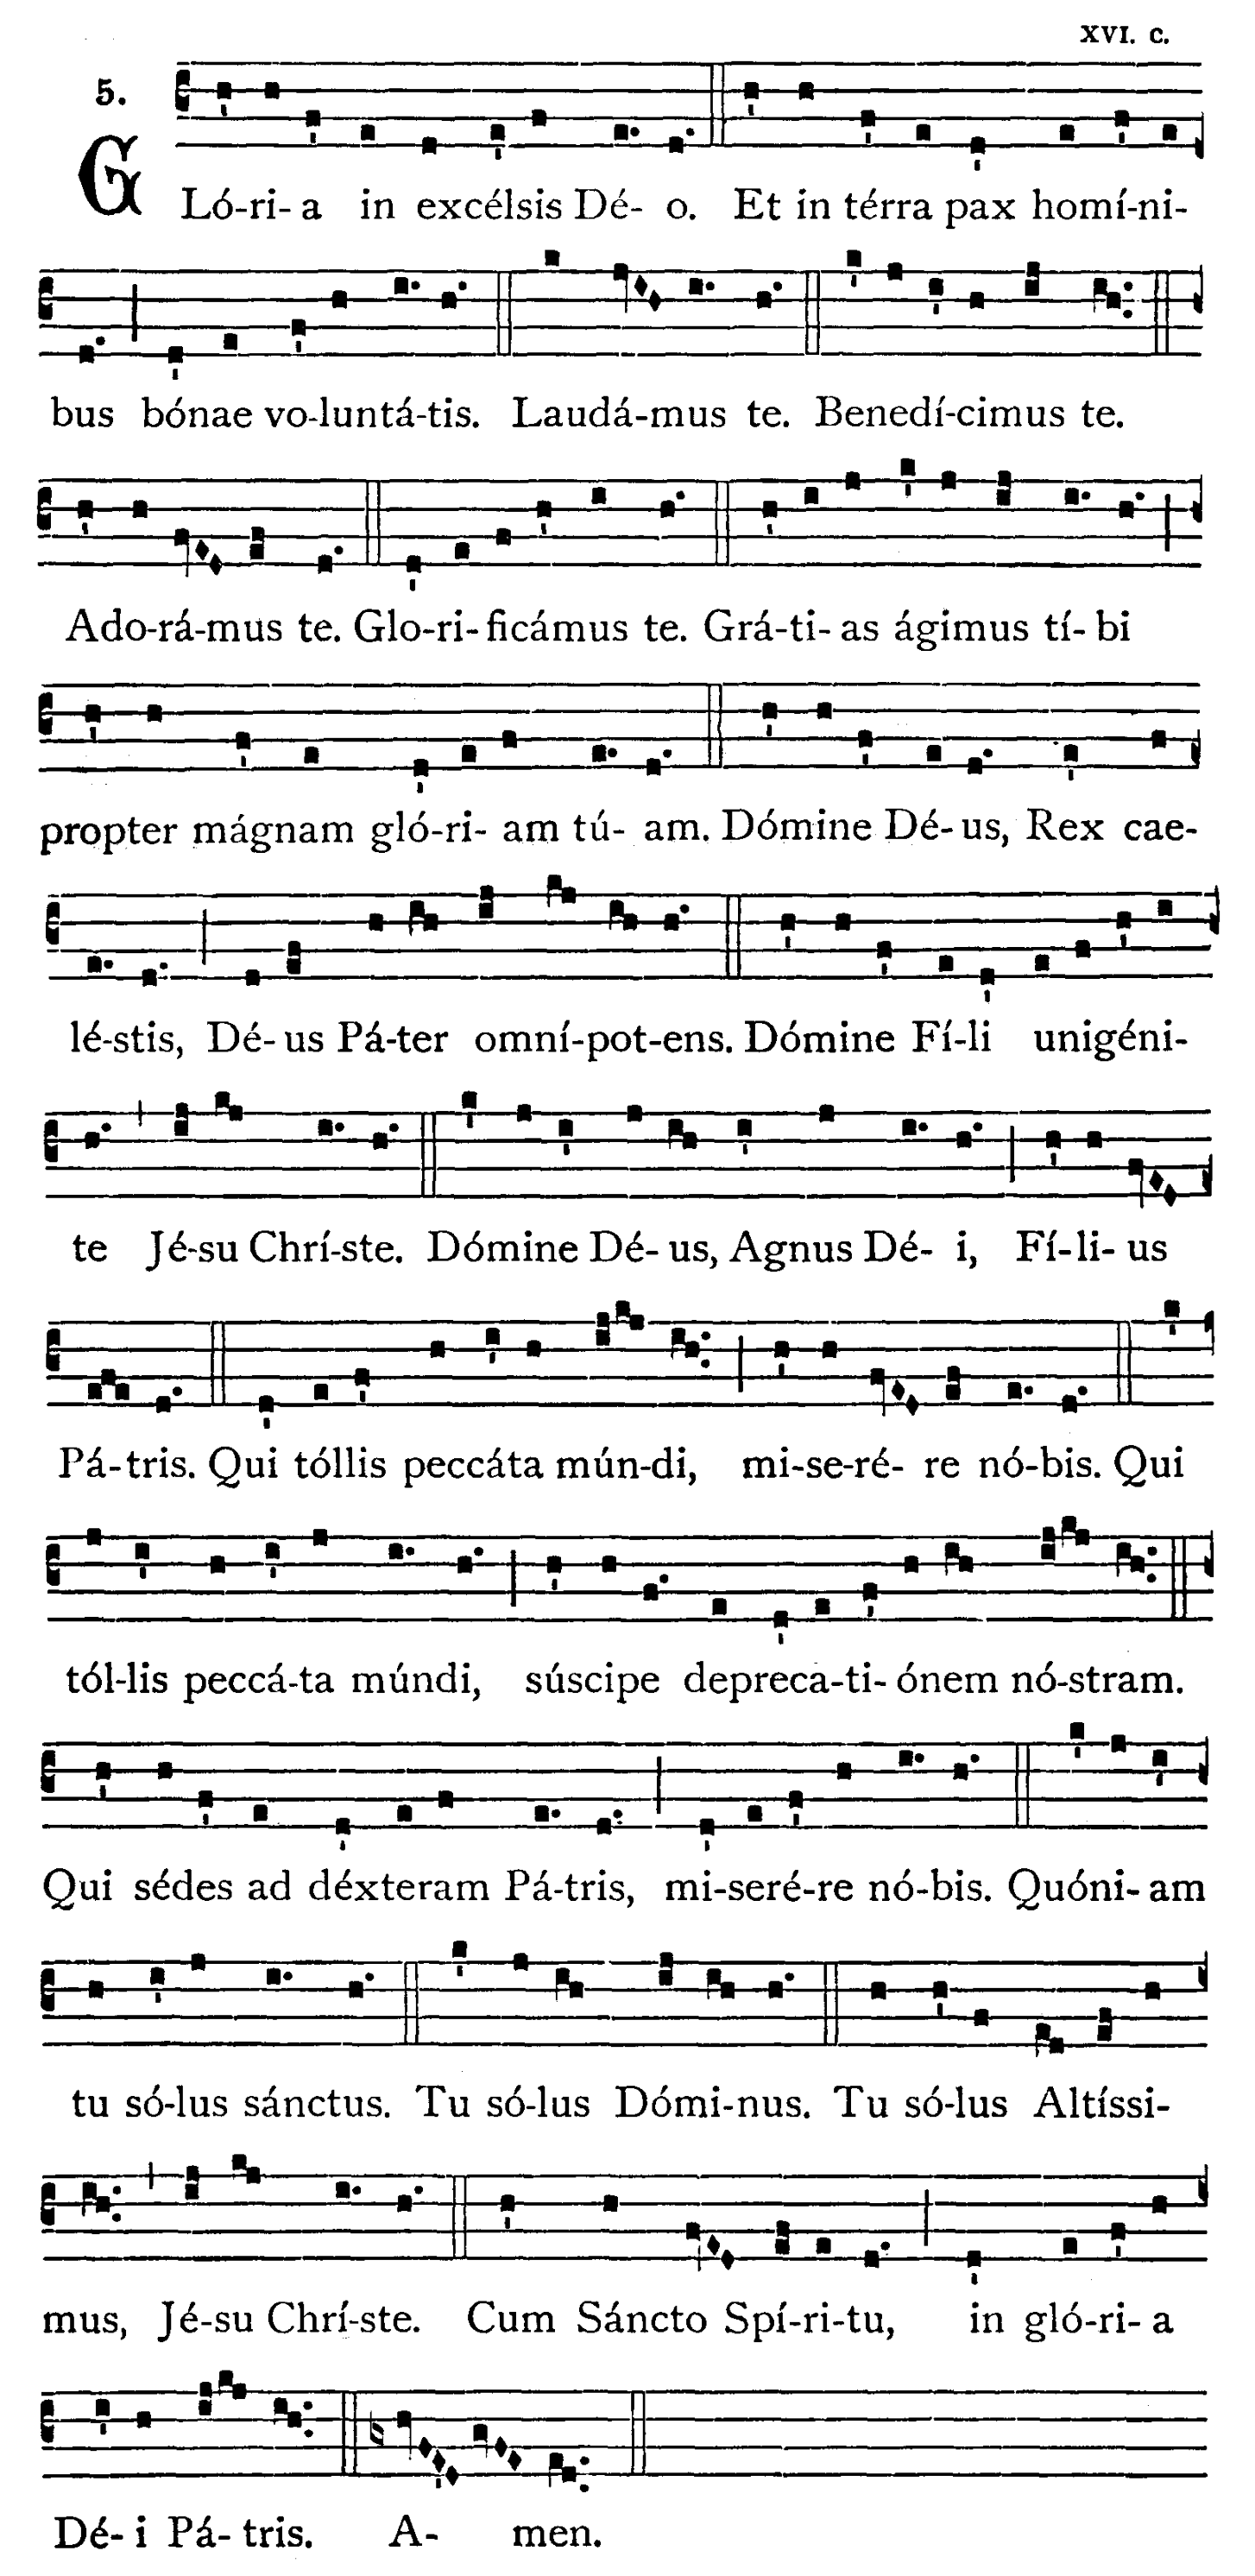
\includegraphics
        [scale=0.3, clip, viewport=3cm 96cm 29cm 103cm]
        {img/gloria.png}
\end{wrapfigure}

\begin{figure}[p]
    \centering
    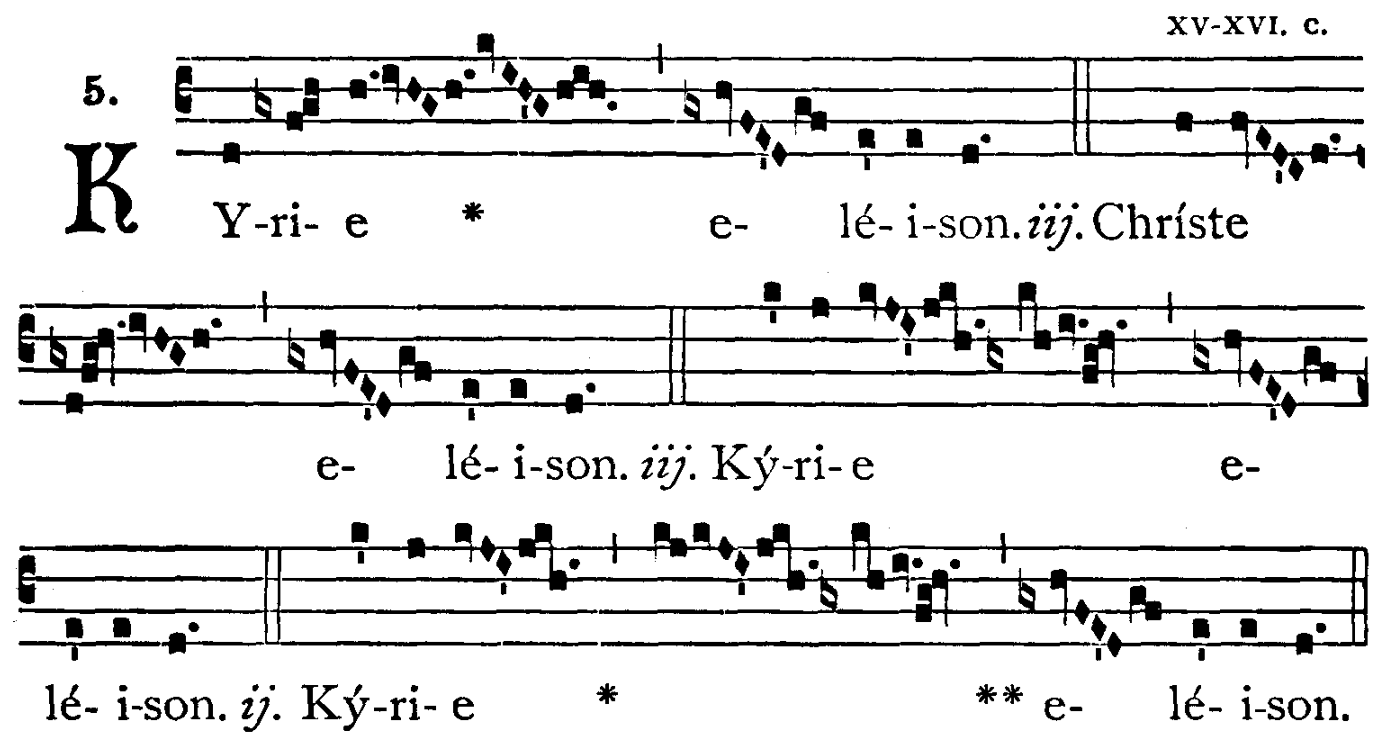
\includegraphics[scale=0.3]{img/kyrie.png}
    \\[2\baselineskip]
    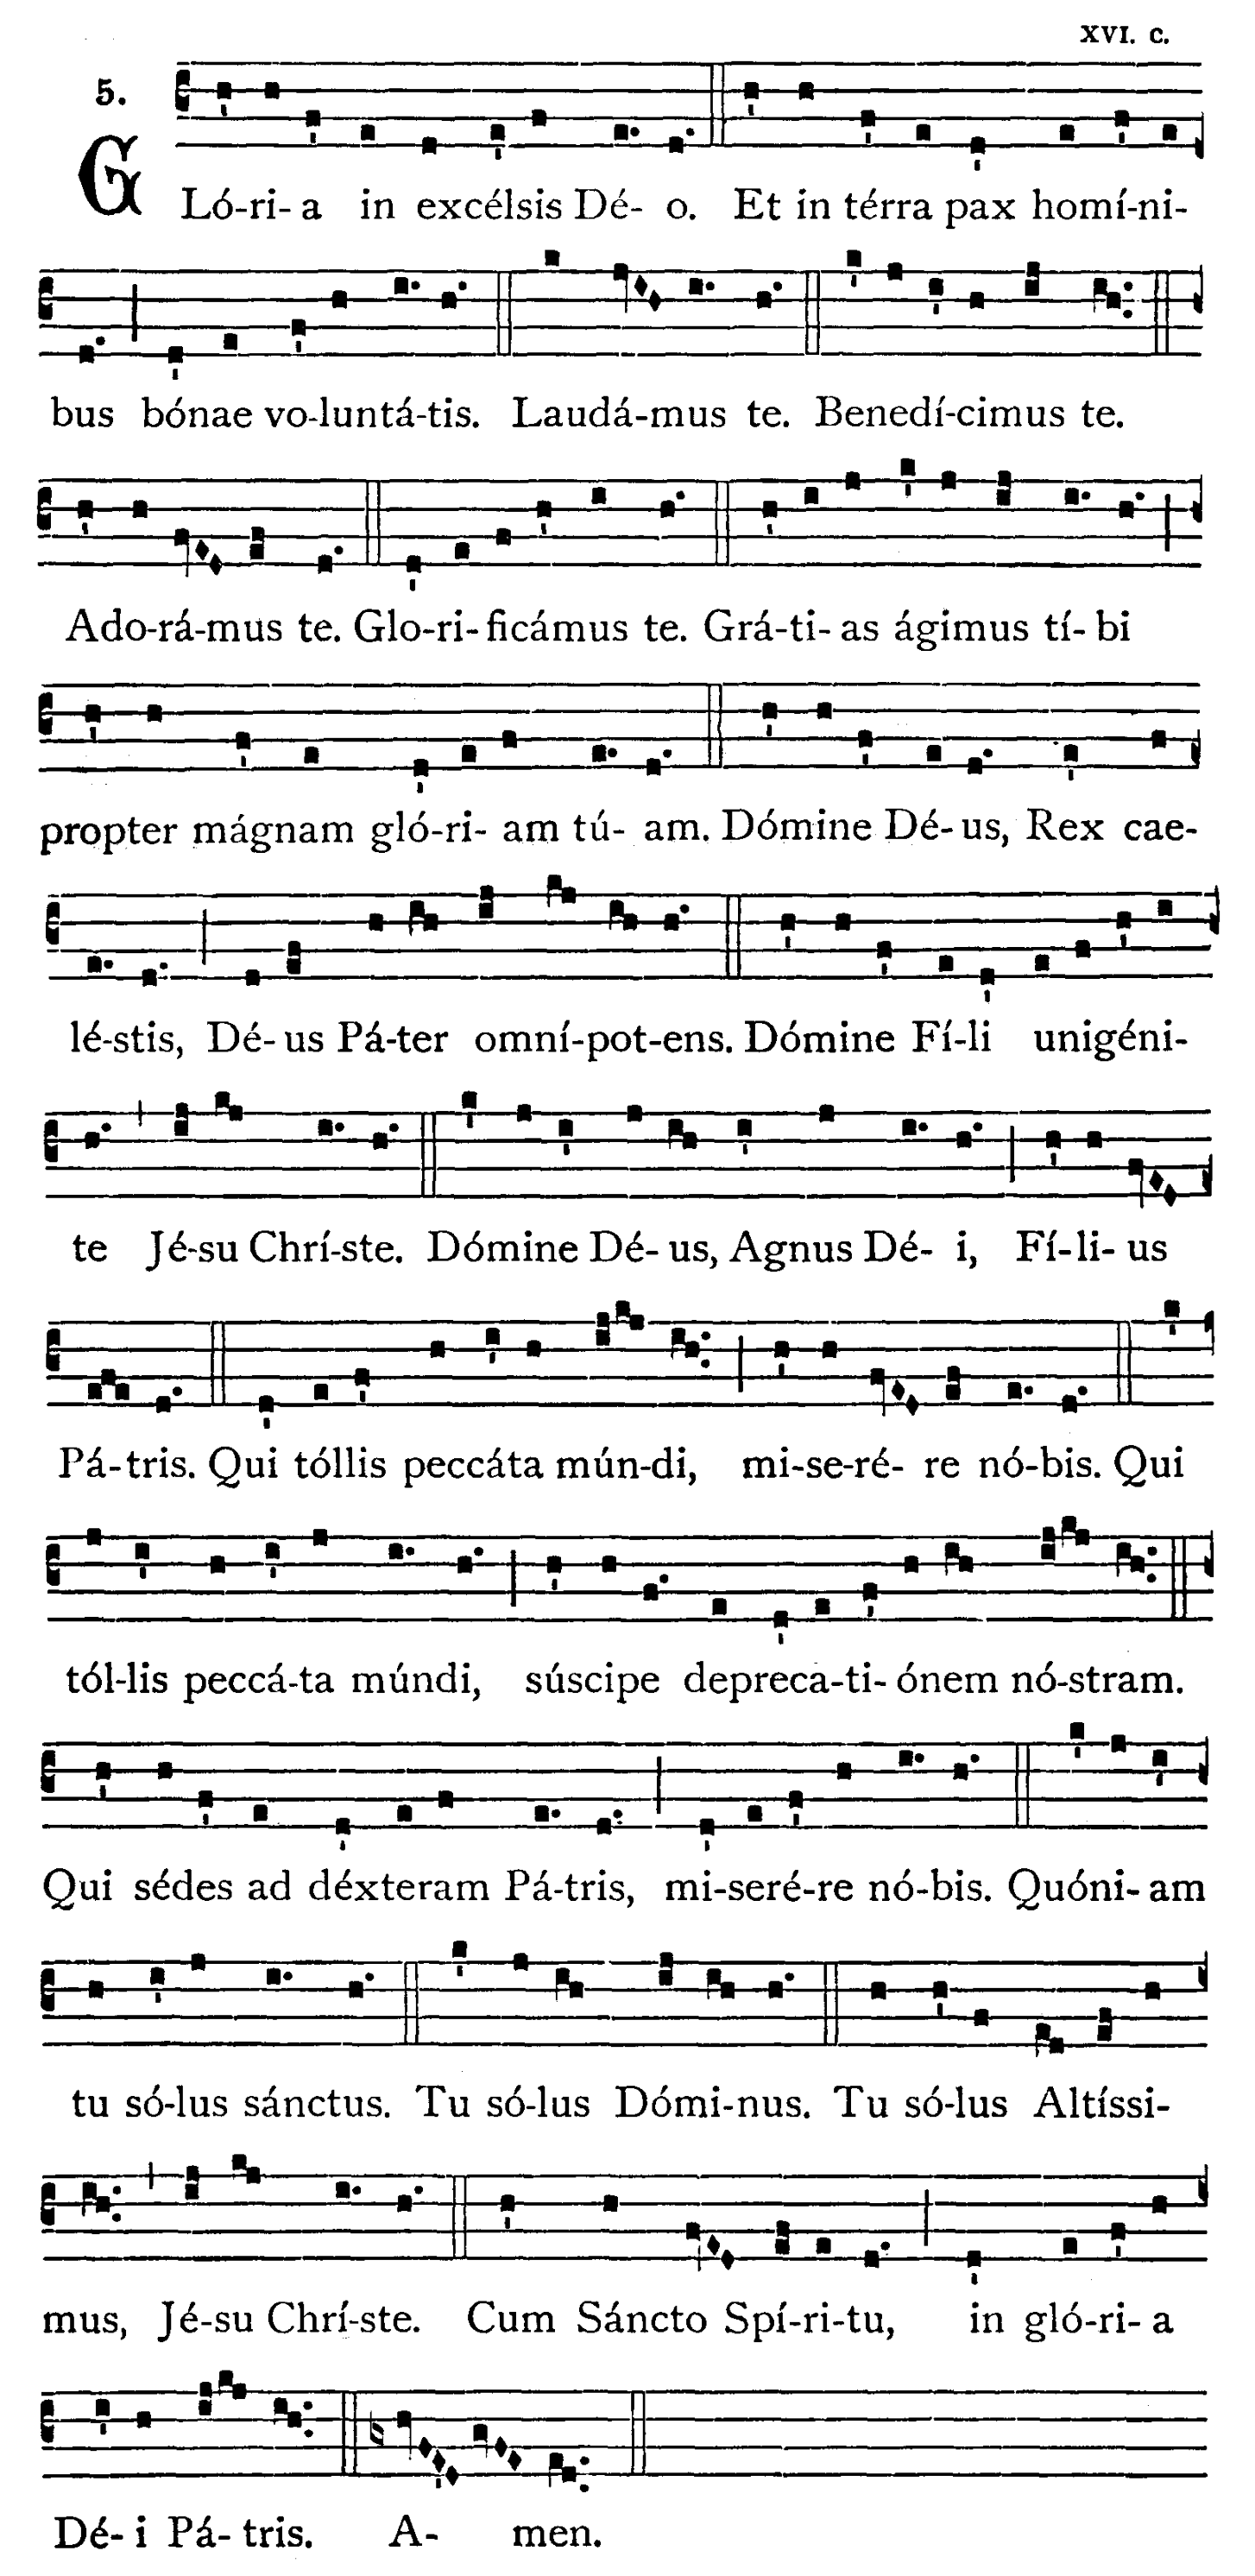
\includegraphics
        [scale=0.3, clip, viewport=1cm 53cm 50cm 105cm]
        {img/gloria.png}
\end{figure}

\begin{figure}[ht]
    \vspace*{2\baselineskip}
    \centering
    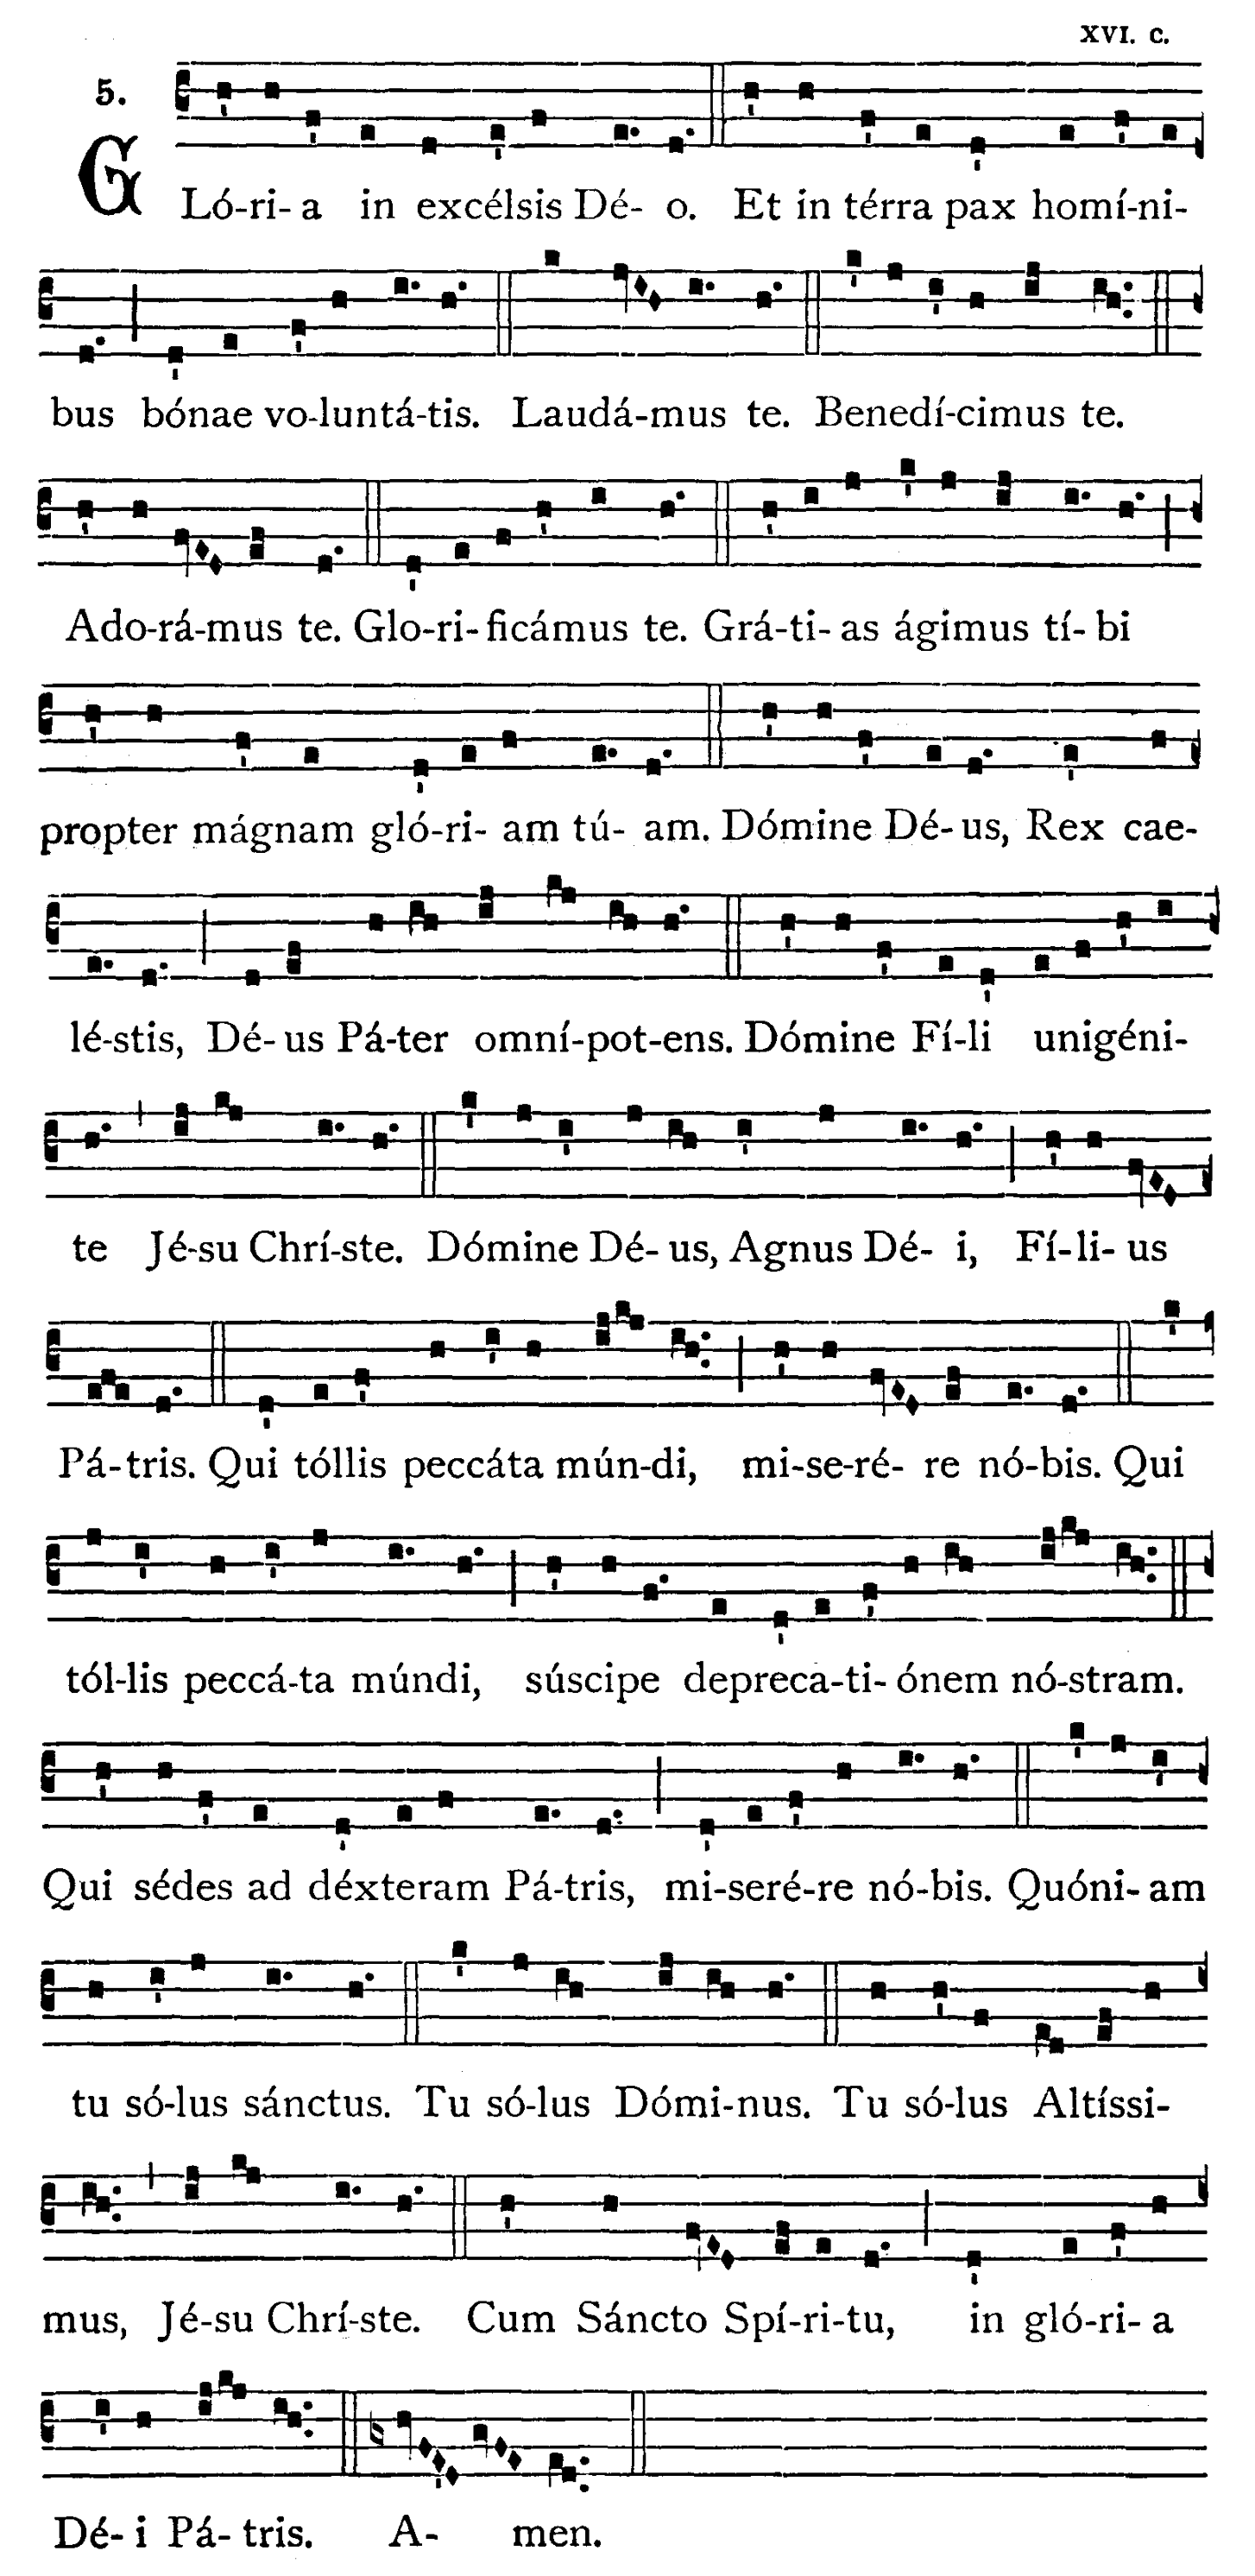
\includegraphics
        [scale=0.3, clip, viewport=1cm 1cm 50cm 53cm]
        {img/gloria.png}
    \vspace*{2\baselineskip}
\end{figure}

\textit{Postea in medio altaris extendens et iungens manus, caputque
aliquantulum inclinans, dicit, si dicendum est}, Gloria in excelsis Deo,
\textit{et prosequitur iunctis manibus.  Cum dicit} Adoramus te, Gratias agimus
tibi, \textit{et} Iesu Christe, et Suscipe deprecationem, \textit{inclinat
caput: et in fine dicens:} Cum Sancto Spiritu, \textit{signat se a fronte ad
pectus.}

\biblia{Lc. 2, 14}

\initialis{G}loria in excelsis Deo.  Et in terra pax hominibus bonae voluntatis.
Laudamus te.  Benedicimus te.  \directio{flectens} Adoramus te.  Glorificamus
te.  \directio{flectens} Gratias agimus tibi propter magnam gloriam tuam.
Domine Deus, Rex caelestis, Deus Pater omnipotens.  Domine Fili unigenite,
\directio{flectens} Iesu Christe.  Domine Deus, Agnus Dei, Filius Patris.  Qui
tollis peccata mundi, miserere nobis.  Qui tollis peccata mundi,
\directio{flectens} suscipe deprecationem nostram.  Qui sedes ad dexteram
Patris, miserere nobis.  Quoniam tu solus Sanctus.  Tu solus Dominus.  Tu solus
Altissimus, \directio{flectens} Iesu Christe.  \cross{} Cum Sancto Spiritu, in
gloria Dei Patris.  Amen.

\textit{Deinde osculatur altare in medio, et versus ad populum dicit:}

\versiculum{Dominus vobiscum.}
\alternatim{\par\responsorium{Et cum spiritu tuo.}}

\textit{Postea dicit:}

\versiculum{Oremus.}

\textit{%
    et orationes, unam aut plures, ut Ordo Officii postulat.  Sequitur Epistola,
    graduale, tractus, vel Alleluia cum versu, aut sequentia, prout Tempus aut
    qualitas Missae postulat.
}

\section{Collecta}

\proprius{Collecta}

\section{Epistola}

\directio{sedens}

\directio{proprius: Epistola}

\section{Graduale, Tractus, Alleluia, Sequentia}

\proprius{Graduale/Tractus/Alleluia/Sequentia}

\section{Evangelium}

\textit{%
    His finitis, si Missa est solemnis, diaconus librum Evangeliorum deponit
    super medium altaris, et, nisi sit Missa defunctorum, celebrans benedicit
    incensum, ut supra: deinde diaconus, genuflexus ante altare, manibus
    iunctis, dicit:
}

\initialis{M}unda cor meum ac labia mea, omnipotens Deus, qui labia Isaiae
prophetae calculo mundasti ignito: ita me tua grata miseratione dignare mundare,
ut sanctum Evangelium tuum digne valeam nuntiare.  Per Christum Dominum nostrum.
Amen.

\textit{%
    Postea accipit librum de altari, et rursus genuflexus petit benedictionem a
    sacerdote, dicens:
}

\versiculum{Iube, domne, benedicere.}

\textit{Sacerdos respondet:}

\initialis{D}ominus sit in corde tuo et in labiis tuis: ut digne et competenter
annunties Evangelium suum: In nomine Patris, Filii, \cross{} et Spiritus Sancti.
Amen.

\directio{stans}

\textit{%
    Et, accepta benedictione, osculatur manum celebrantis: et cum aliis
    ministris, incenso, et luminaribus, accedens ad locum Evangelii, stans
    iunctis manibus, dicit:
}

\versiculum{Dominus vobiscum.}
\alternatim{\par\responsorium{Et cum spiritu tuo.}}

\textit{Et pronuntians:}

\versiculum{Sequentia sancti Evangelii secundum N.}

\textit{sive} Initium, \textit{pollice dexterae manus signat librum in principio
Evangelii, quod est lecturus, deinde seipsum in fronte, ore, et pectore: et dum
ministri respondent:}

\directio{signans se in fronte, ore, et pectore}

\responsorium{Gloria tibi, Domine.}

\textit{incensat ter librum, postea prosequitur Evangelium iunctis manibus.}

\proprius{Evangelium}

\textit{%
    Quo finito, subdiaconus defert librum sacerdoti, qui osculatur Evangelium,
    dicens:
}

\sacerdos{Per evangelica dicta deleantur nostra delicta.}

\textit{Deinde sacerdos incensatur a diacono.}

\divisio

\textit{Si vero sacerdos sine diacono et subdiacono celebrat, delato libro ad
aliud latus altaris, inclinatus in medio, iunctis manibus dicit} Munda cor meum,
\textit{ut supra, et} Iube, Domine, benedicere.  Dominus sit in corde meo
et in labiis meis: ut digne et competenter annuntiem Evangelium suum.  Amen.

\textit{Deinde, conversus ad librum, iunctis manibus, dicit}:

\versiculum{Dominus vobiscum.}
\alternatim{\par\responsorium{Et cum spiritu tuo.}}

\textit{Et pronuntians}:

\versiculum{Initium (\textit{sive} Sequentia) sancti Evangelii.}

\textit{%
    signat librum, et se in fronte, ore, et pectore, et legit Evangelium, ut
    dictum est.  Quo finito, respondet minister:
}

\responsorium{Laus tibi, Christe.}

\textit{et sacerdos osculatur Evangelium, dicens:}

\sacerdos{Per evangelica dicta\ldots (\textit{ut supra})}

\textit{In Missis defunctorum dicitur} Munda cor meum, \textit{sed non petitur
benedictio, non deferuntur luminaria, nec celebrans osculatur librum.}

\divisio

\section{Credo}

\begin{wrapfigure}{r}{0.5\textwidth}
    \centering
    \vspace{-0.5\baselineskip}
    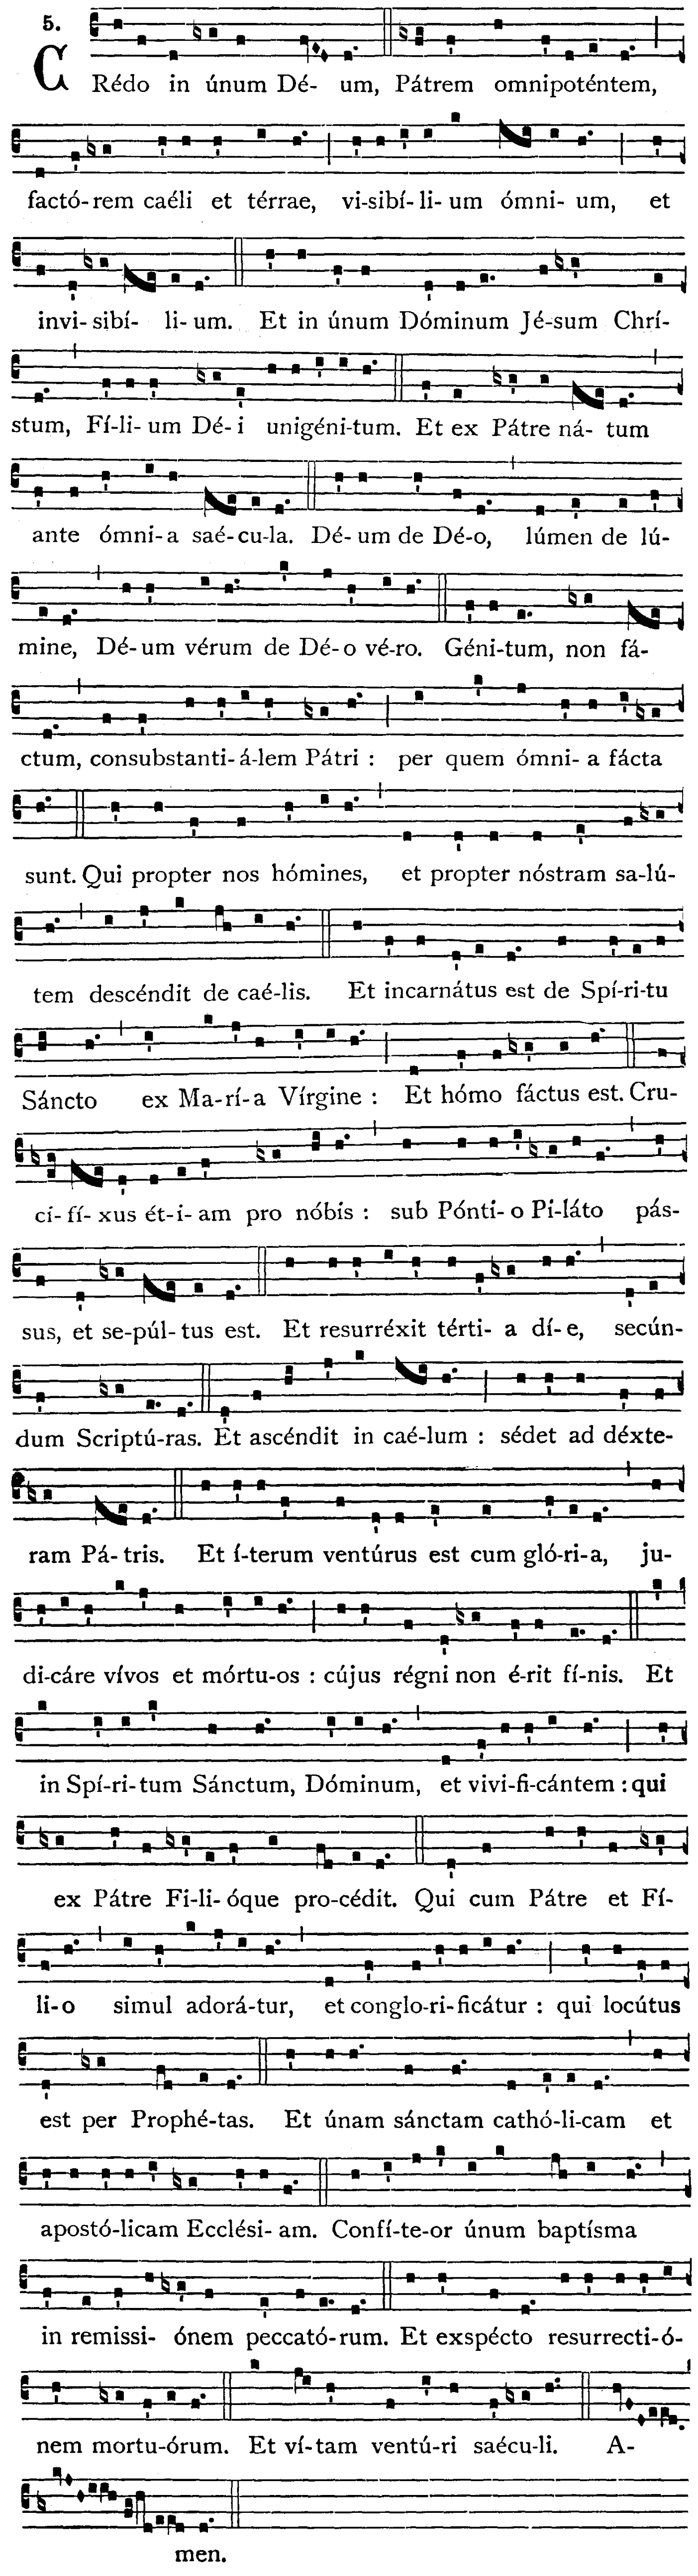
\includegraphics
        [scale=0.3, clip, viewport=2cm 175.5cm 27.25cm 183cm]
        {img/credo.png}
    \vspace{-0.5\baselineskip}
\end{wrapfigure}

\textit{Deinde ad medium altaris extendens, elevans et iungens manus, dicit, si
dicendum est}, Credo in unum Deum, \textit{et prosequitur iunctis manibus.  Cum
dicit} Deum, \textit{caput cruci inclinat: quod similiter facit, cum dicit}
Iesum Christum, \textit{et} simul adoratur.  \textit{Ad illa autem verba} Et
incarnatus est, \textit{genuflectit usque dum dicatur} Et homo factus est.
\textit{In fine ad} Et vitam venturi saeculi, \textit{signat se signo crucis a
fronte ad pectus.}

\initialis{C}redo in unum Deum, Patrem omnipotentem, factorem caeli et terrae,
visibilium omnium et invisibilium.  Et in unum Dominum \directio{flectens} Iesum
Christum, Filium Dei unigenitum.  Et ex Patre natum ante omnia saecula.  Deum de
Deo, lumen de lumine, Deum verum de Deo vero.  Genitum, non factum,
consubstantialem Patri: per quem omnia facta sunt.  Qui propter nos homines et
propter nostram salutem descendit de caelis.  \directio{genuflectens} \textsc{Et
incarnatus est de Spiritu Sancto ex Maria Virgine: et homo factus est}.
Crucifixus etiam pro nobis: sub Pontio Pilato passus, et sepultus est.  Et
resurrexit tertia die, secundum Scripturas.  Et ascendit in caelum: sedet ad
dexteram Patris.  Et iterum venturus est cum gloria iudicare vivos et mortuus:
cuius regni non erit finis.  Et in Spiritum Sanctum, Dominum, et vivificantem:
qui ex Patre Filioque procedit.  Qui cum Patre et Filio \directio{flectens}
simul adoratur et conglorificatur: qui locutus est per Prophetas.  Et unam
sanctam catholicam et apostolicam Ecclesiam.  Confiteor unum baptisma in
remissionem peccatorum.  Et exspecto resurrectionem mortuorum.  \cross{} Et
vitam venturi saeculi.  Amen.

\begin{center}
    \vspace*{\fill}
    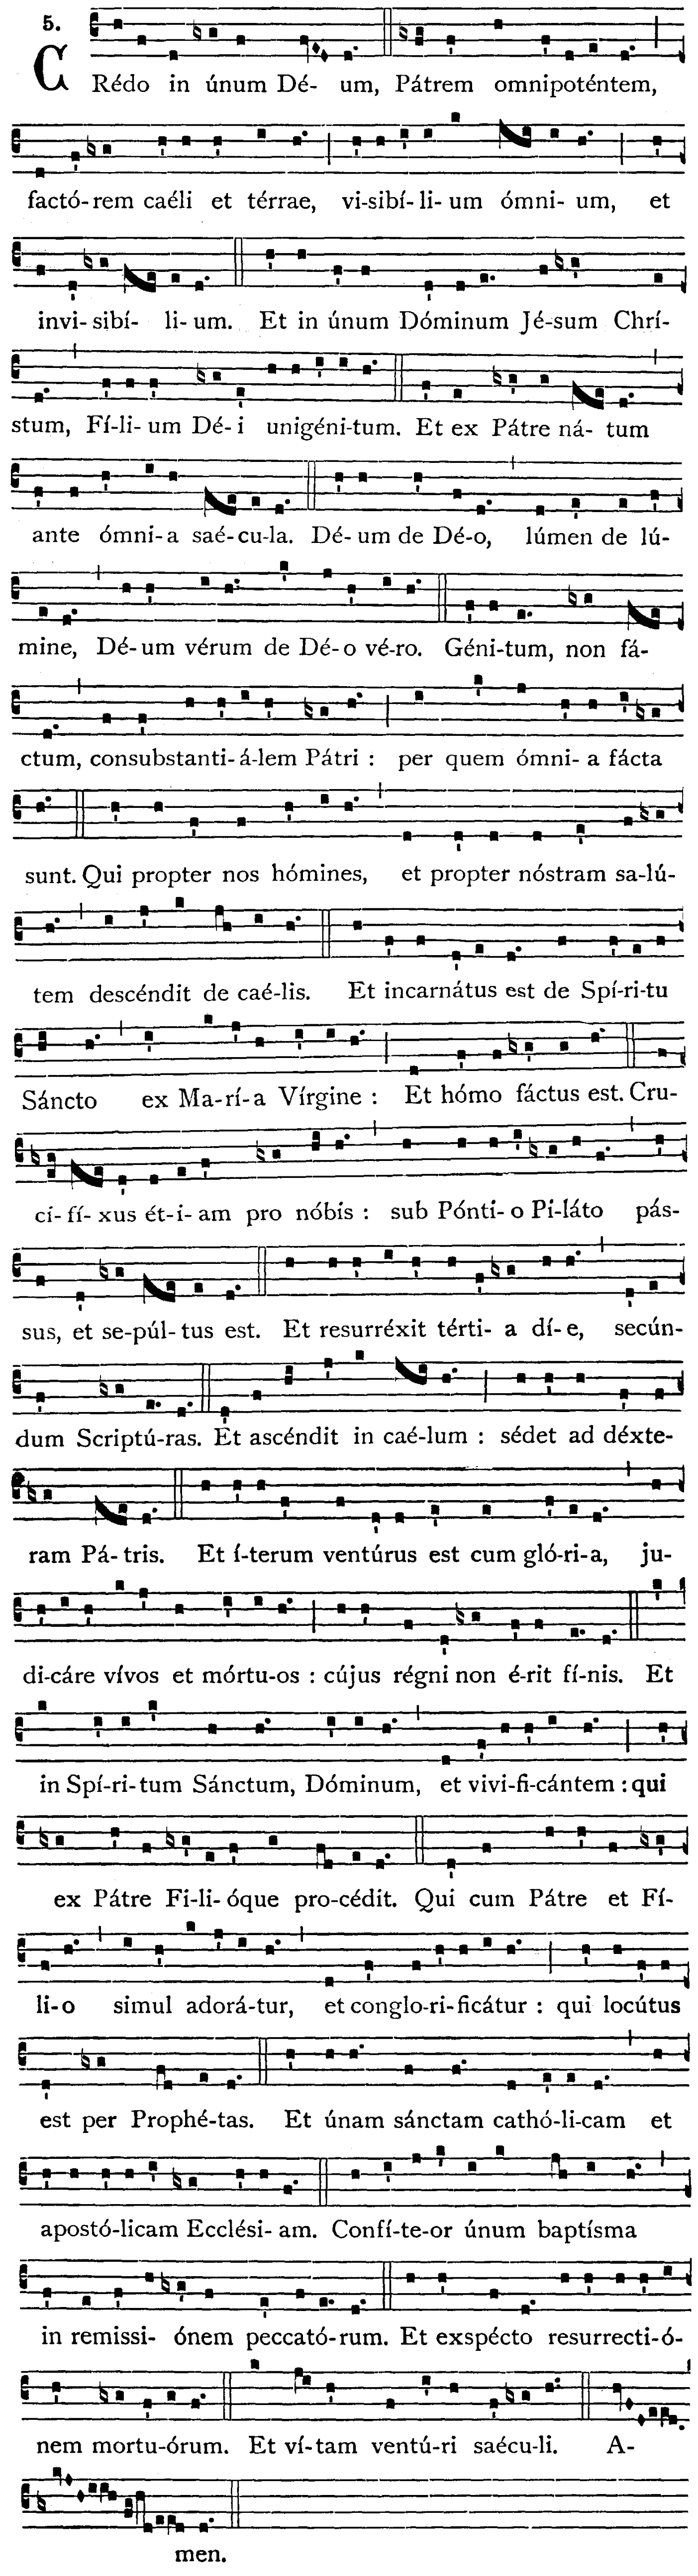
\includegraphics
        [scale=0.3, clip, viewport=0cm 159cm 49.25cm 183cm]
        {img/credo.png}
    \vspace*{\fill}
    \pagebreak
    \vspace*{\fill}
    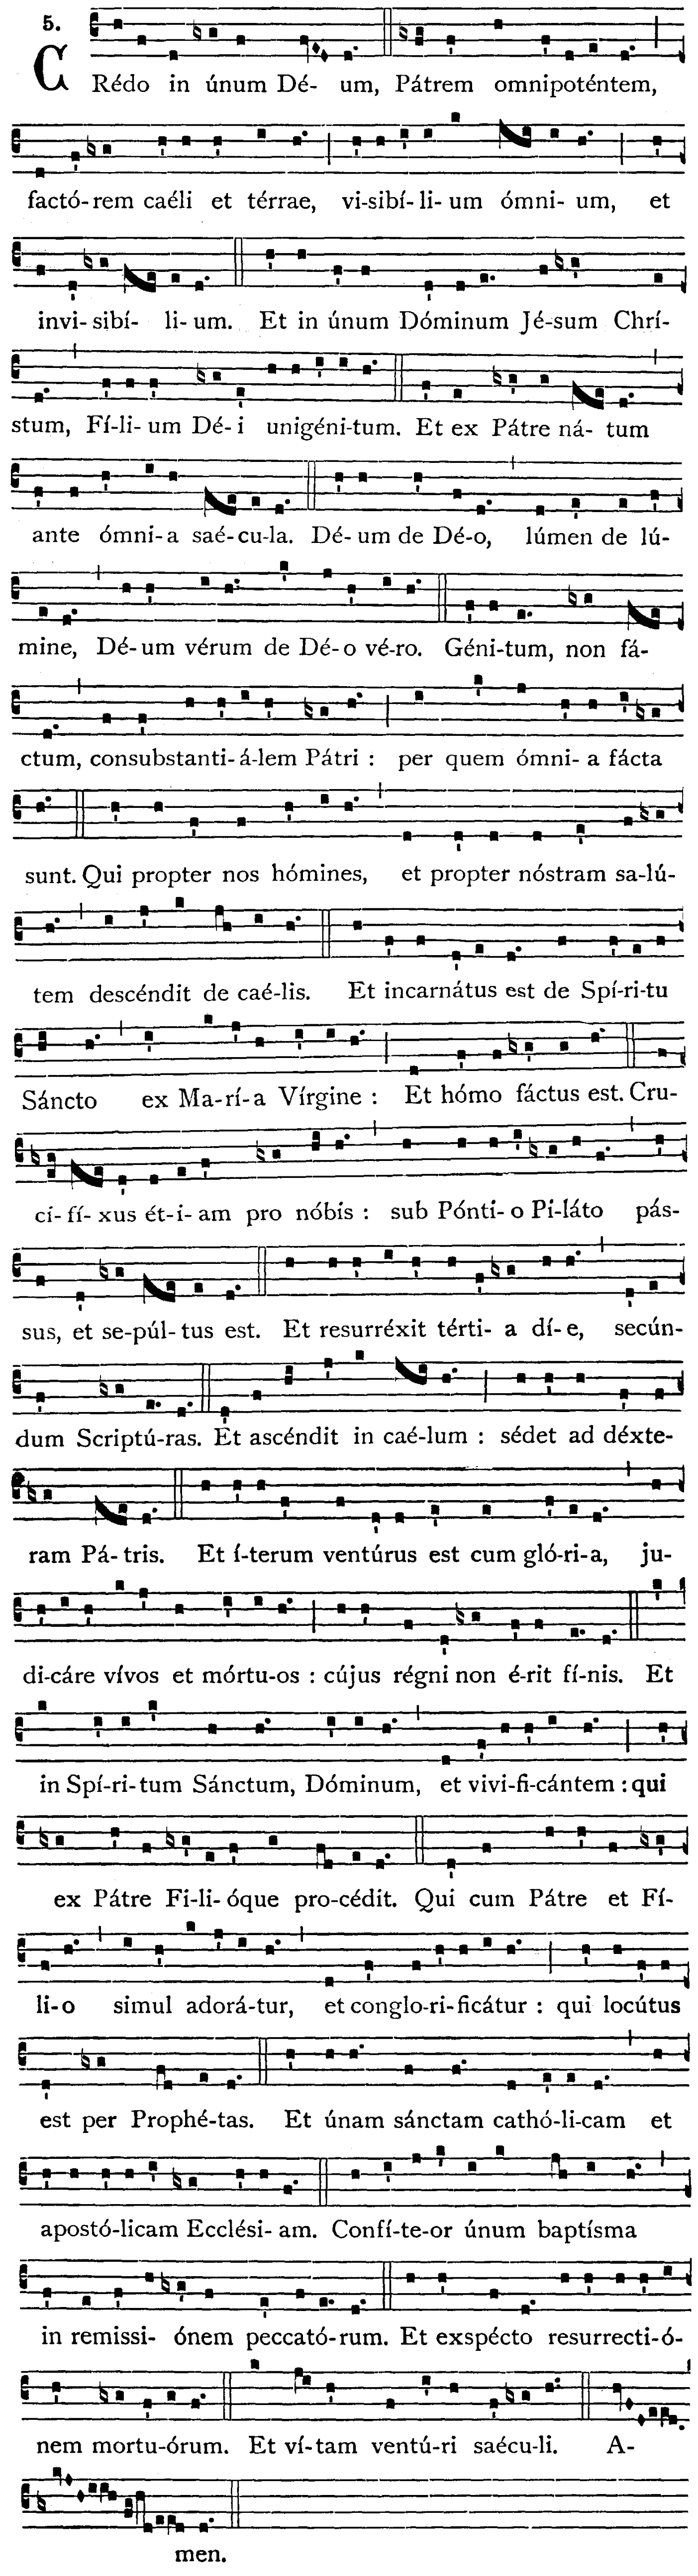
\includegraphics
        [scale=0.3, clip, viewport=0cm 80cm 49.25cm 158cm]
        {img/credo.png}
    \vspace*{\fill}
    \pagebreak
    \vspace*{\fill}
    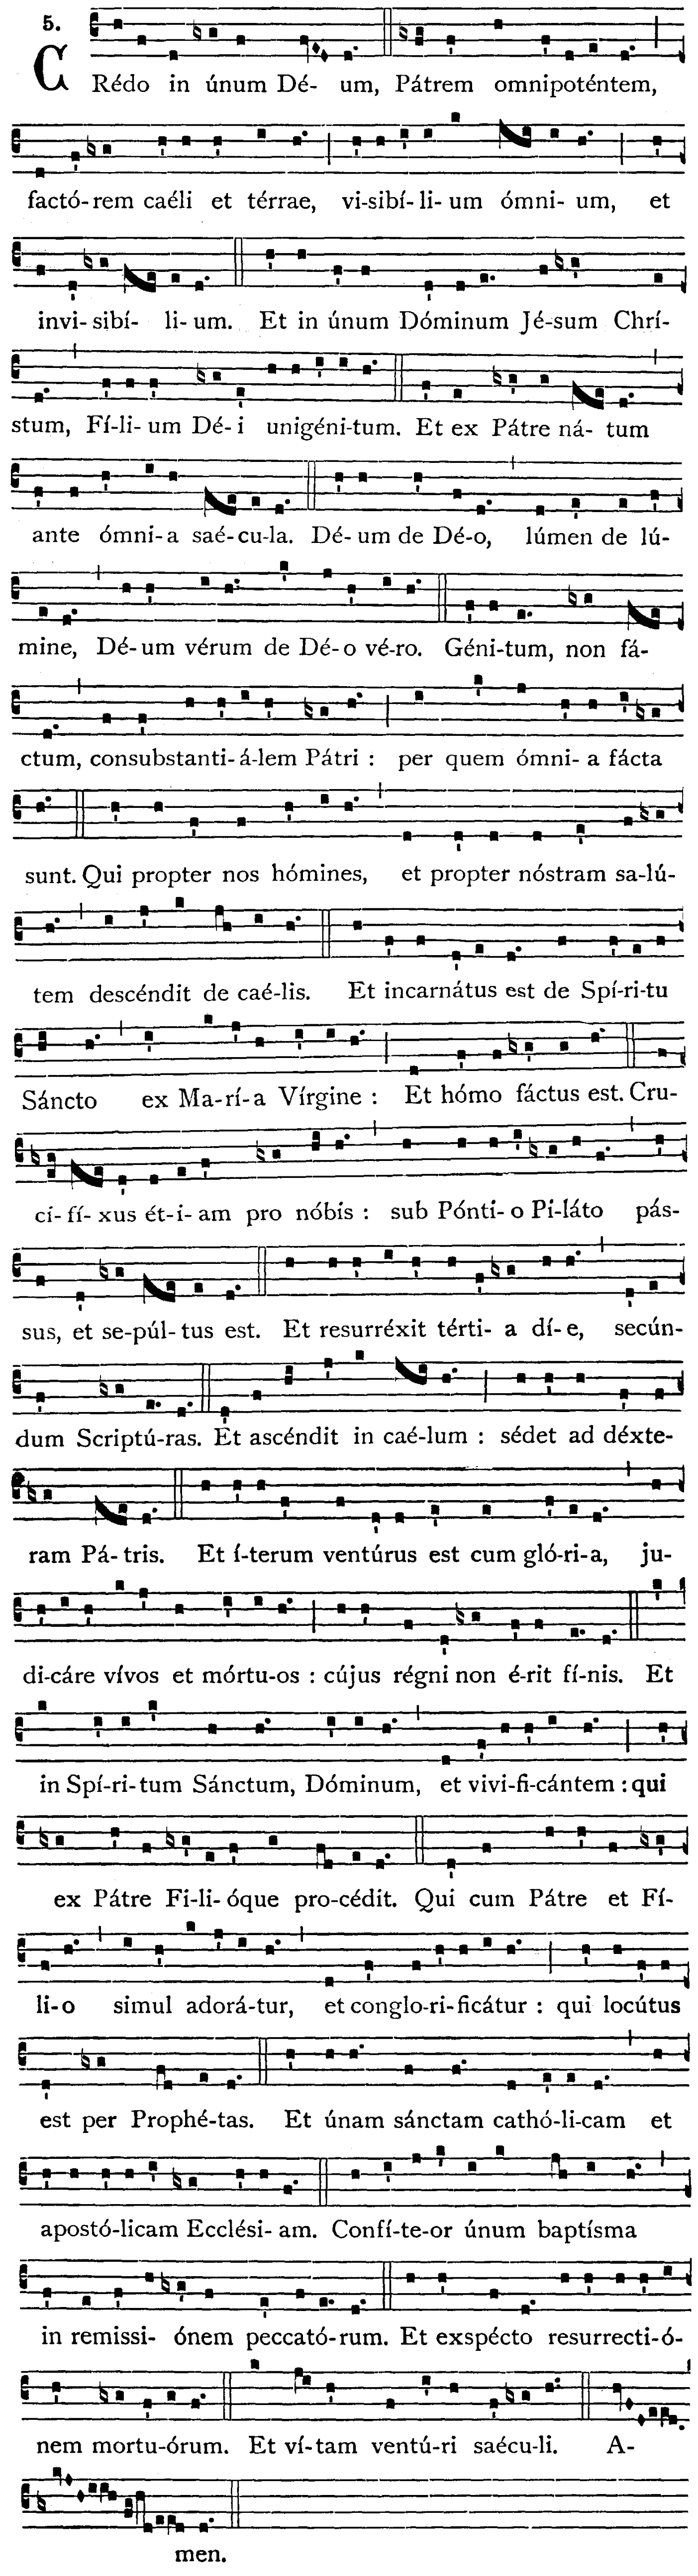
\includegraphics
        [scale=0.3, clip, viewport=0cm 0cm 49.25cm 79cm]
        {img/credo.png}
    \vspace*{\fill}
\end{center}

    {\let\cleardoublepage\clearpage\chapter{Missa Fidelium}}

\directio{stans}

\textit{Deinde osculatur altare, et, versus ad populum, dicit:}

\versiculum{Dominus vobiscum.}
\alternatim{\par\responsorium{Et cum spiritu tuo.}}

\textit{Postea dicit}:

\versiculum{Oremus.}

\textit{et antiphonam ad Offertorium.}

\section{Offertorium}

\directio{sedens}

\proprius{Offertorium}

\textit{%
    Qua dicta, si est Missa solemnis, diaconus porrigit celebranti patenam cum
    hostis: secus sacerdos ipse accipit patenam cum hostia, quam offerens,
    dicit:
}

\initialis{S}uscipe, sancte Pater, omnipotens aeterne Deus, hanc immaculatam
hostiam, quam ego indignus famulus tuus offero tibi Deo meo vivo et vero, pro
innumerabilibus peccatis, et offensionibus, et neglegentiis meis, et pro omnibus
circumstantibus, sed et pro omnibus fidelibus christianis vivis atque defunctis:
ut mihi et illis proficiat ad salutem in vitam aeternam.  Amen.

\textit{%
    Deinde faciens crucem cum eadem patena, deponit hostiam super corporale.
    Diaconus ministrat vinum, subdiaconus aquam in calice: vel si Missa sine
    sacris ministris celebratur, utrumque infundit sacerdos, et aquam miscendam
    in calice benedicit signo crucis, dicens:
}

\initialis{D}eus, qui humanae substantiae dignitatem mirabiliter, condidisti, et
mirabilius reformasti: da nobis, per huius aquae et vini mysterium, eius
divinitatis esse consortes, qui humanitatis nostrae fieri dignatus est
particeps, Iesus Christus; Filius tuus, Dominus noster: Qui tecum vivit et
regnat in unitate Spiritus Sancti Deus: per omnia saecula saeculorum.  Amen.

\divisio

\textit{%
    In Missis defunctorum dicitur praedicta oratio: sed aqua non
    benedicitur.
}

\divisio

\textit{Postea accipit calicem, et offert, dicens}:

\initialis{O}fferimus tibi, Domine, calicem salutaris, tuam deprecantes
clementiam: ut in conspectu divinae maiestatis tuae, pro nostra et totius mundi
salute, cum odore suavitatis ascendat.  Amen.

\textit{%
    Deinde facit signum crucis cum calice, et illum ponit super corporale, et
    palla cooperit: tum, iunctis manibus super altare, aliquantulum inclinatus,
    dicit:
}

\biblia{Dn. 3, 39}

\initialis{I}n spiritu humilitatis et in animo contrito suscipiamur a te,
Domine: et sic fiat sacrificium nostrum in conspectu tuo hodie, ut placeat tibi,
Domine Deus.

\textit{%
    Erectus expandit manus, easque in altum porrectas iungens, elevatis ad
    caelum oculis, et statim demissis, dicit:
}

\initialis{V}eni, sanctificator omnipotens aeterne Deus: (\textit{benedicit
oblata, prosequendo:}) et bene\cross{}dic hoc sacrificium, tuo sancto nomini
praeparatum.

\section{Incensum}

\textit{Postea, si solemniter celebrat, benedicit incensum, dicens}:

\initialis{P}er intercessionem beati Michaelis Archangeli, stantis a dextris
altaris incensi, et omnium electorum suorum, incensum istud dignetur Dominus
bene\cross{}dicere, et in odorem suavitatis accipere.  Per Christum Dominum
nostrum.  Amen.

\textit{%
    Et, accepto thuribulo a diacono, incensat oblata, modo in rubricis
    praescripto, dicens:
}

\initialis{I}ncensum istud a te benedictum ascendat ad te, Domine: et descendat
super nos misericordia tua.

\textit{Deinde incensat altare, dicens}:

\biblia{Ps. 140, 2-4}

\initialis{D}irigatur, Domine, oratio mea, sicut incensum, in conspectu tuo:
elevatio manuum mearum sacrificium vespertinum.  Pone, Domine, custodiam ori
meo, et ostium circumstantiae labiis meis: ut non declinet cor meum in verba
malitiae, ad excusandas excusationes in peccatis.

\textit{Dum reddit thuribulum diacono, dicit}:

\initialis{A}ccendat in nobis Dominus ignem sui amoris et flammam aeternae
caritatis.  Amen.

\textit{Postea incensatur sacerdos a diacono, deinde alii per ordinem.}

\directio{stans ad incensionem}

\section{Lavatio}

\textit{Interim sacerdos lavat manus, dicens:}

\biblia{Ps. 25, 6-12}

\initialis{L}avabo inter innocentes manus meas: et circumdabo altare tuum,
Domine: Ut audiam vocem laudis, et enarrem universa mirabilia tua.  Domine,
dilexi decorem domus tuae, et locum habitationis gloriae tuae.  Ne perdas cum
impiis, Deus, animam meam, et cum viris sanguinum vitam meam: In quorum manibus
iniquitates sunt: dextera eorum repleta est muneribus.  Ego autem in innocentia
mea ingressus sum: redime me, et miserere mei.  Pes meus stetit in directo: in
ecclesiis benedicam te, Domine.  Gloria Patri, et Filio, et Spiritui Sancto.
Sicut erat in principio, et nunc, et semper: et in saecula saeculorum.  Amen.

\divisio

\textit{%
    In Missis defunctorum, et tempore Passionis in Missis de Tempore omittitur
    Gloria Patri.
}

\divisio

\section{Sancta Trinitas}

\textit{%
    Deinde, aliquantulum inclinatus in medio altaris, iunctis manibus super eo,
    dicit:
}

\initialis{S}uscipe, sancta Trinitas, hanc oblationem, quam tibi offerimus ob
memoriam passionis, resurrectionis et ascensionis Iesu Christi Domini nostri: et
in honorem beatae Mariae semper Virginis, et beati Ioannis Baptistae, et
sanctorum Apostolorum Petri et Pauli, et istorum, et omnium Sanctorum: ut illis
proficiat ad honorem, nobis autem ad salutem: et illi pro nobis intercedere
dignentur in caelis, quorum memoriam agimus in terris.  Per eundem Christum
Dominum nostrum.  Amen.

\section{Orate Fratres}

\textit{%
    Postea osculatur altare et, versus ad populum, extendens et iungens manus,
    voce paululum elevata, dicit:
}

\initialis{O}rate, fratres: ut meum ac vestrum sacrificium acceptabile fiat apud
Deum Patrem omnipotentem.

\textit{Minister, seu circumstantes respondet: alioquin ipsemet sacerdos}:

\initialis{S}uscipiat Dominus sacrificium de manibus tuis (\textit{vel meis}) ad
laudem et gloriam nominis sui, ad utilitatem quoque nostram, totiusque Ecclesiae
suae sanctae.

\textit{Sacerdos submissa voce dicit:}

\sacerdos{Amen.}

\section{Secreta}

\textit{Deinde, manibus extensis, absolute sine} Oremus \textit{subiungit
orationes secretas.}

\proprius{Secreta}

\textit{Quibus finitis, cum pervenerit ad conclusionem, clara voce dicit}:

\versiculum{Per omnia saecula saeculorum}
\alternatim{\par\responsorium{Amen.}}

\textit{cum praefatione, ut in sequentibus}.

\section{Praefatio}

\directio{stans}

\textit{Praefationem incipit ambabus manibus positis hinc inde super altare:
quae aliquantulum elevat, cum dicit}: Sursum corda.  \textit{Iungit eas ante
pectus, et caput inclinat, cum dicit}: Gratias agamus Domino Deo nostro.
\textit{Deinde disiungit manus, et disiunctas tenet usque ad finem
praefationis:}

\versiculum{Dominus vobiscum.}
\alternatim{%
    \par\responsorium{Et cum spiritu tuo.}
    \par\versiculum{Susrum corda.}
    \par\responsorium{Habemus ad Dominum.}
    \par\versiculum{Gratias agamus Domino Deo nostro.}
    \par\responsorium{Dignum et iustum est.}
}

\proprius{Praefatio}

\initialis{V}ere dignum et iustum est, aequum et salutare, nos tibi semper, et
ubique gratias agere: Domine sancte, Pater omnipotens, aeterne Deus: Qui cum
unigenito Filio tuo, et Spiritu Sancto, unus es Deus, unus es Dominus: non in
unius singularitate personae, sed in unius Trinitate substantiae.  Quod enim de
tua gloria, relevante te, credimus, hoc de Filio tuo, hoc de Spiritu Sancto,
sine differentia discretionis sentimus.  Ut in confessione verae, sempiternaeque
Deitatis, et in personis proprietas, et in essentia unitas, et in maiestate
adoretur aequalitas.  Quam laudant Angeli atque Archangeli, Cherubim quoque ac
Seraphim: qui non cessant clamare quotidie, una voce dicens:

\section{Sanctus}

\directio{genuflectens}

\textit{qua finita, iterum iungit eas, et inclinatus dicit}: Sanctus.
\textit{Et cum dicit}: Benedictus qui venit, \textit{signum crucis sibi producit
a fronte ad pectus}.

\sinus

{
    \Large\centering
    \par Sanctus, sanctus, sanctus, Dominus Deus Sabaoth.  Plani sunt caeli et
    terra gloria tua.
    \par Hosanna in excelsis.
    \par Bene\cross{}dictus qui venit in nomine Domini.
    \par Hosanna in excelsis.
    \par
}

\section{Canon}

\textit{%
    Finita praefatione, sacerdos, extendes, elevans aliquantulum et iungens
    manus, elevansque ad caelum oculos, et statim demittens, profunde inclinatus
    ante altare, manibus super eo positis, dicit secreto:
}

\initialis{T}e igitur, clementissime Pater, per Iesum Christum, Filium tuum,
Dominum nostrum, supplices rogamus ac petimus (\textit{osculatur altare et,
iunctis manibus ante pectus dicit:}) uti accepta habeas et benedicas
(\textit{signat ter super hostiam et calicem simul, dicens:}) haec \cross{}
dona, haec \cross{} munera, haec \cross{} sancta sacrificia illibata
(\textit{extensis manibus prosequitur:}) in primis, quae tibi offerimus pro
Ecclesia tua sancta catholica: quam pacificare, custodire, adunare et regere
digneris toto orbe terrarum: una cum famulo tuo Papa nostro \textit{N.} et
Antistite nostro \textit{N.} et omnibus orthodoxis, atque catholicae et
apostolicae fidei cultoribus.

\subsection{Commemoratio pro vivis}

\initialis{M}emento, Domine, famulorum famularumque tuarum \textit{N.} et
\textit{N.} (\textit{iungit manus, orat aliquantulum pro quibus orare intendit:
deinde manibus extensis prosequitur:}) et omnium circumstantium, quorum tibi
fides cognita est et nota devotio, pro quibus tibi offerimus: vel qui tibi
offerunt hoc sacrificium laudis, pro se suisque omnibus: pro redemptione
animarum suarum, pro spe salutis et incolumitatis suae: tibique reddunt vota sua
aeterno Deo, vivo et vero.

\subsection{Infra Actionem}

\initialis{C}ommunicantes, et memoriam venerantes, in primis gloriosae semper
Virginis Mariae, Genetricis Dei et Domini nostri Iesu Christi: sed et beati
Ioseph, eiusdem Virginis Sponsi, et beatorum Apostolorum ac Martyrum tuorum,
Petri et Pauli, Andreae, Iacobi, Ioannis, Thomae, Iacobi, Philippi,
Bartholomaei, Matthaei, Simonis et Thaddaei: Lini, Cleti, Clementis, Xysti,
Cornelii, Cypriani, Laurentii, Chrysogoni, Ioannis et Pauli, Cosmae et Damiani:
et omnium Sanctorum tuorum; quorum meritis precibusque concedas, ut in omnibus
protectionis tuae muniamur auxilio.  (\textit{iungit manus}) Per eundem Christum
Dominum nostrum.  Amen.

\subsection{Hanc Igitur}

\textit{Tenens manus expansas super oblata, dicit:}

\sinus

\initialis{H}anc igitur oblationem servitutis nostrae, sed et cunctae familiae
tuae, quaesumus, Domine, ut placatus accipias: diesque nostros in tua pace
disponas, atque ab aeterna damnatione nos eripi, et in electorum tuorum iubeas
grege numerari.  (\textit{iungit manus}) Per Christum Dominum nostrum.  Amen.

\subsection{Quam Oblationem}

\initialis{Q}uam oblationem tu, Deus, in omnibus, quaesumus (\textit{signat ter
super oblata}) bene\cross{}dictam, adscrip\cross{}tam, ra\cross{}tam,
rationabilem, acceptabilemque facere digneris: (\textit{signat semel super
hostiam}) ut nobis Cor\cross{}pus, (\textit{et semel super calicem}) et
San\cross{}guis fiat dilectissimi Filii tui (\textit{iungit manus}) Domini
nostri Iesu Christi.

\initialis{Q}ui pridie quam pateretur (\textit{accipit hostiam}) accepit panem
in sanctas ac venerabiles manus suas: (\textit{elevat oculos ad caelum}) et
elevatis oculis in caelum ad te Deum Patrem suum omnipotentem (\textit{caput
inclinat}) tibi gratias agens, (\textit{signat super hostiam})
bene\cross{}dixit, fregit, deditque discipulis suis, dicens: Accipite, et
manducate ex hoc omnes.

\textit{%
    Tenens ambabus manibus hostiam inter indices et pollices, profert verba
    consecrationis distincte et attente super hostiam, et simul super omnes, si
    plures sint consecrandae.
}

\biblia{Lc. 22, 19-20}

{\Large\centering Hoc est enim Corpus meum.\par}

\sinus\sinus\sinus

\textit{%
    Quibus verbis prolatis, statim hostiam consecratam genuflexus adorat:
    surgit, ostendit populo, reponit super corporale, et genuflexus iterum
    adorat: nec amplius pollices et indices disiungit, nisi quando hostia
    tractanda est, usque ad ablutionem digitorum.  Tunc, detecto calice, dicit:
}

\initialis{S}imili modo postquam cenatum est (\textit{ambabus manibus accipit
calicem}), accipiens et hunc praeclarum calicem in sanctas ac venerabiles manus
suas: item (\textit{caput inclinat}) tibi gratias agens, (\textit{sinistra
tenens calicem, dextera signat super eum}) bene\cross{}dixit, deditque
discipulis suis, dicens: Accipite, et bibite ex eo omnes.

\textit{%
    Profert verba consecrationis super calicem attente et continuate, tenens
    illum parum elevatum.
}

{
    \Large\centering
    Hic est enim Calix Sanguinis mei, novi et aeterni testamenti: mysterium
    fidei: qui pro vobis et pro multis effundetur in remissionem peccatorum.
    \par
}

\sinus\sinus\sinus

\textit{Quibus verbis prolatis, deponit calicem super corporale, et dicens:}

{\Large\centering Haec quotiescumque feceritis, in mei memoriam facietis.\par}

\textit{%
    genuflexus adorat: surgit, ostendit populo, deponit, cooperit, et genuflexus
    iterum adorat.  Deinde, disiunctis manibus, dicit:
}

\initialis{U}nde et memores, Domine, nos servi tui, sed et plebs tua sancta,
eiusdem Christi Filii tui, Domini nostri, tam beatae passionis, nec non et ab
inferis resurrectionis, sed et in caelos gloriosae ascensionis: offerimus
praeclarae maiestati tuae de tuis donis ac datis, (\textit{iungit manus, et
signat ter super hostiam et calicem simul, dicens:}) hostiam \cross{} puram,
hostiam \cross{} sanctam, hostiam \cross{} immaculata, (\textit{signat semel
super hostiam, dicens:}) Panem \cross{} sanctum vitae aeternae, (\textit{et
semel super calicem, dicens:}) et Calicem \cross{} salutis perpetuae.

\textit{Extensis manibus prosequitur:}

\initialis{S}upra quae propitio ac sereno vultu respicere digneris: et accepta
habere, sicuti accepta habere dignatus es munera pueri tui iusti Abel, et
sacrificium Patriarchae nostri Abrahae: et quod tibi obtulit summus sacerdos
tuus Melchisedech, sanctum sacrificium, immaculatam hostiam.

\textit{Profunde inclinatus, iunctis manibus et super altare positis, dicit:}

\initialis{S}upplices te rogamus, omnipotens Deus: iube haec perferri per manus
sancti Angeli tui in sublime altare tuum, in cospectu divinae maiestatis tuae:
ut, quotquot, (\textit{osculatur altare}) ex hac altaris participatione
sacrosanctum Filii tui (\textit{iungit manus, et signat semel super hostiam, et
semel super calicem}) Cor\cross{}pus et San\cross{}guinem sumpserimus
(\textit{seipsum signat, dicens:}) omni benedictione caelesti et gratia
repleamur.  (\textit{Iungit manus}) Per eundem Christum Dominum nostrum.  Amen.

\subsection{Commemoratio pro defunctis}

\initialis{M}emento etiam, Domine, famulorum famularumque tuarum \textit{N.} et
\textit{N.}, qui nos praecesserunt cum signo fidei, et dormiunt in somno pacis.

\textit{%
    Iungit manus, orat aliquantulum pro iis defunctis, pro quibus orare
    intendit, deinde extensis manibus prosequitur:
}

Ipsis, Domine, et omnibus in Christo quiescentibus, locum refrigerii, lucis et
pacis, ut indulgeas, deprecamur.  (\textit{Iungit manus et caput inclinat,
dicens:}) Per eundem Christum Dominum nostrum.  Amen.

\textit{Manu dextera percutit sibi pectus, elata aliquantulum voce dicens:}

\initialis{N}obis quoque peccatoribus (\textit{extensis manibus ut prius,
secrete prosequitur:}) famulis tuis, de multitudine miserationum tuarum
sperantibus, partem aliquam et societatem donare digneris, cum tuis sanctis
Apostolis et Martyribus: cum Ioanne, Stephano, Matthia, Barnaba, Ignatio,
Alexandro, Marcellino, Petro, Felicitate, Perpetua, Agatha, Lucia, Agnete,
Caecilia, Anastasia, et omnibus Sanctis tuis: intra quorum nos consortium, non
aestimator meriti, sed veniae, quaesumus, largitor admitte.  (\textit{Iungit
manus}) Per Christum Dominum nostrum.

\subsection{Doxologia finalis et elevatio minor}

\initialis{P}er quem haec omnia, Domine, semper bona creas, (\textit{signat ter
super hostiam et calicem simul, dicens:}) sancti\cross{}ficas,
vivi\cross{}ficas, bene\cross{}dicis et praestas nobis.

\textit{%
    Discooperit calicem, genuflectit, accipit hostiam inter pollicem et indicem
    manus dexterae: et tenens sinistra calicem, cum hostia signat ter a labio ad
    labium calicis, dicens:
}

Per ip\cross{}sum, et cum ip\cross{}so, et in ip\cross{}so, (\textit{cum ipsa
hostia signat bis inter se et calicem, dicens:}) est tibi Deo Patri \cross{}
omnipotenti, in unitate Spiritus \cross{} Sancti, (\textit{elevans parum calicem
cum hostia, dicit:}) omnis honor, et gloria.

\textit{%
    Reponit hostiam, calicem palla cooperit, genuflectit, surgit, et dicit
    intellegibili voce vel cantat:
}

\directio{stans}

\versiculum{Per omnia saecula saeculorum.}
\alternatim{\par\responsorium{Amen.}}

\subsection{Pater Noster}

\textit{Iungit manus.}

\versiculum{%
    Oremus.  Praeceptis salutaribus moniti, et divina instituitione formati,
    audemus dicere:
}

\textit{Extendit manus.}

\initialis{P}ater noster, qui es in caelis: sanctificetur nomen tuum: adveniat
regnum tuum: Fiat voluntas tua, sicut in caelo, et in terra.  Panem nostrum
cotidianum da nobis hodie: Et dimitte nobis debita nostra, sicut et nos
dimittimus debitoribus nostris.  Et ne nos inducas in tentationem.

\responsorium{Sed libera nos a malo.}

\textit{Sacerdos secrete dicit:}

\versiculum{Amen.}

\textit{%
    Deinde manu dextera accipit inter indicem et medium digitos patenam, quam
    tenens super altare erectam, dicit secrete:
}

\initialis{L}ibera nos, quaesumus Domine, ab omnibus malis, praeteritis,
prasentibus et futuris: et intercedente beata et gloriosa semper Virgine Dei
Genetrice Maria, cum beatis Apostolis tuis Petro et Paulo, atque Andrea, et
omnibus Sanctis, (\textit{signat se cum patena a fronte ad pectus}) da propitius
pacem in diebus nostris: (\textit{patenam osculatur}) ut, ope misericordiae tuae
adiuti, et a peccato simus semper liberi et ab omni perturbatione securi.

\subsection{Fracto Panis}

\textit{%
    Submittit patenam hostiae, discooperit calicem, genuflectit, surgit, accipit
    hostiam, et eam super calicem tenens utraque manu, frangit per medium,
    dicens:
}

{\Large\centering Per eundem Dominum nostrum Iesum Christum, Filium tuum.\par}

\textit{%
    Et mediam partem, quam in dextera manu tenet, ponit super patenam.  Deinde
    ex parte, quae in sinistra remanserat, frangit particulam, dicens:
}

{
    \Large\centering
    Qui tecum vivit et regnat in unitate Spiritus Sancti Deus.
    \par
}

\textit{%
    Aliam mediam partem, quam in sinistra manu habet, adiungit mediae super
    patenam positae, et particulam parvam dextera retinens super calicem, quem
    sinistra per nodum infra cuppam tenet, dicit intellegibili voce vel cantat:
}

\versiculum{Per omnia saecula saeculorum.}
\alternatim{\par\responsorium{Amen.}}

\subsection{Commixtio Corporis et Sanguinis}

\textit{Cum ipsa particula signat ter super calicem, dicens:}

\versiculum{Pax \cross{} Domini sit \cross{} semper vobis\cross{}cum.}
\alternatim{\par\responsorium{Et cum spiritu tuo.}}

\textit{Particulam ipsam immittit in calicem, dicens secrete:}

\initialis{H}aec commixtio, et consecratio Corporis et Sanguinis Domini nostri
Iesu Christi, fiat accipientibus nobis in vitam aeternam.  Amen.

\section{Agnus Dei}

\directio{genuflectens}

\textit{%
    Cooperit calicem, genuflectit, surgit, et inclinatus Sacramento, iunctis
    manibus, et per pectus percutiens, intellegibili voce dicit:
}

{
    \Large\centering
    \par Agnus Dei, qui tollis peccata mundi: miserere nobis.
    \par Agnus Dei, qui tollis peccata mundi: miserere nobis.
    \par Agnus Dei, qui tollis peccata mundi: dona nobis pacem.
    \par
}

\divisio

\textit{In Missis defunctorum non dicitur} miserere nobis, \textit{sed eius
loco} dona eis requiem, \textit{et in tertio additur} sempiternam.

\divisio

\textit{%
    Deinde, iunctis manibus super altare, inclinatus dicit secrete sequentes
    orationes:
}

\initialis{D}omine Iesu Christe, qui dixisti Apostolis tuis: Pacem relinquo
vobis, pacem meam do vobis: ne respicias peccata mea, sed fidem Ecclesiae tuae;
eamque secundum voluntatem tuam pacificare et coadunare digneris: Qui vivis et
regnas Deus per omnia saecula saeculorum.  Amen.

\textit{Si danda est pax, osculatur altare et, dans pacem, dicit:}

\versiculum{Pax tecum.}
\alternatim{\par\responsorium{Et cum spiritu tuo.}}

\divisio

\textit{In Missis defunctorum non datur pax, neque dicitur praecedens oratio.}

\divisio

\initialis{D}omine Iesu Christe, Fili Dei vivi, qui ex voluntate Patris,
cooperante Spiritu Sancto, per mortem tuam mundum vivificasti: libera me per hoc
sacrosanctum Corpus et Sanguinem tuum ab omnibus iniquitatibus meis et universis
malis: et fac me tuis semper inhaerere mandatis, et a te numquam separari
permittas: Qui cum eodem Deo Patre et Spiritu Sancto vivis et regnas Deus in
saecula saeculorum.  Amen.

\initialis{P}erceptio Corporis tui, Domine Iesu Christe, quod ego indignus
sumere praesumo, non mihi proveniat in iudicium et condemnationem: sed pro tua
pietate prosit mihi ad tutamentum mentis et corporis, et ad medelam
percipiendam: Qui vivis et regnas cum Deo Patre in unitate Spiritus Sancti Deus,
per omnia saecula saeculorum.  Amen.

\section{Communio}

\textit{Genuflectit, surgit, et dicit:}

\initialis{P}anem caelestem accipiam, et nomen Domini invocabo.

\textit{%
    Deinde parum inclinatus, accipit ambas partes hostiae inter pollicem et
    indicem sinistrae manus, et patenam inter eundem indicem et medium supponit,
    et dextera tribus vicibus percutiens pectus, elata aliquantulum voce, ter
    dicit devote et humiliter:
}

\sinus\sinus\sinus

\biblia{Mt. 8, 8}

\initialis{D}omine, non sum dignus (\textit{et secrete prosequitur:}) ut intres
sub tectum meum: sed tantum dic verbo, et sanabitur anima mea.

\subsection{Communio Fidelis}

\textit{Postea, dextera se signans cum hostia super patenam, dicit:}

\initialis{C}orpus Domini nostri Iesu Christi custodiat animam meam in vitam
aeternam.  Amen.

\textit{%
    Et, se inclinans, reverenter sumit ambas partes hostiae: quibus sumptis,
    deponit patenam super corporale, et erigens se iungit manus, et quiescit
    aliquantulum in meditatione sanctissimi Sacramenti.  Deinde discooperit
    calicem, genuflectit, colligit fragmenta, si quae sint, extergit patenam
    super calicem, interim dicens:
}

\biblia{Ps. 115, 12-13}

\initialis{Q}uid retribuam Domino pro omnibus quae retribuit mihi?  Calicem
salutaris accipiam, et nomen Domini invocabo.

\biblia{Ps. 18, 3}

Laudans invocabo Dominum, et ab inimicis meis salvus ero.

\textit{Accipit calicem manu dextera et, eo se signans, dicit:}

\initialis{S}anguis Domini nostri Iesu Christi custodiat animam meam in vitam
aeternam.  Amen.

\textit{%
    Et, sinistra supponens patenam calici, reverenter sumit totum Sanguinem cum
    particula.  Quo sumpto, si qui sunt communicandi, eos communicet, antequam
    se purificet.
}

\versiculum{Ecce Agnus Dei, ecce qui tollit peccata mundi.}
\alternatim{%
    \par\responsorium{%
        Domine, non sum dignis, ut intres sub tectum meum: sed tantum dic verbo,
        et sanabitur anima mea.
    }
}

\initialis{C}orpus Domini nostri Iesu Christi custodiat animam tuam in vitam
aeternam.

\vspace{0.5\baselineskip}\responsorium{Amen.}

\textit{Postea dicit:}

\initialis{Q}uod ore sumpsimus, Domine, pura mente capiamus: et de munere
temporali fiat nobis remedium sempiternum.

\textit{%
    Interim porrigit calicem ministro, qui infundit in eo parum vini, quo se
    purificat: deinde prosequitur:
}

\initialis{C}orpus tuum, Domine, quod sumpsi, et Sanguis, quem potavi, adhaereat
visceribus meis: et praesta; ut in me non remaneat scelerum macula, quem pura et
sancta refecerunt sacramenta: Qui vivis et regnas in saecula saeculorum.  Amen.

\subsection{Oratio Communionis}

\textit{%
    Abluit et extergit digitos, ac sumit ablutionem: extergit os et calicem,
    quem, plicato corporali, operit et collocat in altari ut prius: deinde
    prosequitur Missam.
}

\proprius{Communio}

\versiculum{Dominus vobiscum.}
\alternatim{%
    \par\responsorium{Et cum spiritu tuo.}
    \par\versiculum{Oremus.}
}

\section{Post Communionem}

\directio{stans}

\proprius{Post Communionem}

\textit{Dicto, post ultimam orationem,}

\versiculum{Dominus vobiscum.}
\alternatim{\par\responsorium{Et cum spiritu tuo.}}

\textit{dicit}

\versiculum{Ite, missa est.}

\divisio

\textit{Vel, si qua liturgica processio sequatur:}

\versiculum{Benedicamus Domino.}

\divisio

\responsorium{Deo gratias.}

\divisio

\textit{In Missis defunctorum dicit:}

\versiculum{Requiescant in pace}
\alternatim{\par\responsorium{Amen.}}

\divisio

\textit{%
    Tunc celebrans inclinat se ante medium altaris, et, manibus iunctis super
    illud, dicit secrete:
}

\initialis{P}laceat tibi, sancta Trinitas, obsequium servitutis meae: et
praesta: ut sacrificium, quod oculis tuae maiestatis indignus obtuli, tibi sit
acceptabile, mihique et omnibus, pro quibus illud obtuli, sit, te miserante,
propitiabile.  Per Christum Dominum nostrum.  Amen.

\subsection{Benedictio}

\textit{%
    Deinde osculatur altare: et elevatis oculis, extendens, elevans et iungens
    manus caputque Cruci inclinans, dicit:
}

\versiculum{Benedicat vos omnipotens Deus.}

\textit{%
    Et versus ad populum, semel tantum benedicens, etiam in Missis solemnibus,
    prosequitur:
}

\versiculum{Pater, et Filius, \cross{} et Spiritus Sanctus.}
\alternatim{\par\responsorium{Amen.}}

\divisio

\textit{In Missa pontificali ter benedicitur, ut in Pontificali habetur.}

\textit{In Missis in quibus dictum est} Benedicamus Domino \textit{vel}
Requiescant in pace, \textit{non datur benedictio, sed dicto} Placeat \textit{et
osculato altari, celebrans legit, si dicendum sit, Evangelium S. Ioannis.}

\divisio

\subsection{Evangelium Secundum Ioannem}

\directio{stans}

\textit{Deinde sacerdos in latere Evangelii, iunctis manibus dicit:}

\versiculum{Dominus vobiscum.}
\alternatim{\par\responsorium{Et cum spiritu tuo.}}

\textit{%
    Et signans signo crucis primum altare vel librum, deinde se in fronte, ore
    et pectore, dicit:
}

{{\liturgicalfont\fontsize{48}{48}\selectfont\raisebox{-0.3em}{᛭}}}
Initium sancti Evangelii secundum Ioannem.

\textit{Vel si aliud Evangelium legendum sit}: Sequentia sancti Evangelii
\textit{etc.}

\responsorium{Gloria tibi, Domine.}

\textit{Iunctis manibus prosequitur:}

\biblia{Io 1, 1-14}

\initialis{I}n principio erat Verbum, et Verbum erat apud Deum, et Deus erat
Verbum.  Hoc erat in principio apud Deum.  Omnia per ipsum facta sunt: et sine
ipso factum est nihil, quod factum est: in ipso vita erat, et vita erat lux
hominum: et lux in tenebris lucet, et tenebrae eam non comprehenderunt.

Fuit homo missus a Deo, cui nomen erat Ioannes.  Hic venit in testimonium, ut
testimonium perhiberet de lumine, ut omnes crederent per illum.  Non erat ille
lux, sed ut testimonium perhiberet de lumine.

Erat lux vera, quae illuminat omnem hominem venientem in hunc mundum.  In mundo
erat, et mundus per ipsum factus est, et mundus eum non cognovit.  In propria
venit, et sui eum non receperunt.  Quotquot autem receperunt eum, dedit eis
potestatem filios Dei fieri, his, qui credunt in nomine eius: qui non ex
sanguinibus, neque ex voluntate carnis, neque ex voluntate viri, sed ex Deo nati
sunt.  (\textit{Genuflectit dicens:}) \textsc{Et Verbum caro factum est}
(\textit{et surgens prosequitur:}) et habitavit in nobis: et vidimus gloriam
eius, gloriam quasi Unigeniti a Patre, plenum gratiae et veritatis.

\responsorium{Deo gratias.}

\end{document}
